%% Intended to be included into a larger document
\chapter{Related Work}
\label{cha:related-work}

This chapter examines research related to serious games and gamification, sustainability, frameworks, and framework assessment. Section \ref{sec:rel-seriousgame} discusses related work on serious games and recent development in gamification. Section \ref{sec:rel-sg-sustainability} looks at the applications of ``serious game'' in the sustainability context. Finally, Section \ref{sec:rel-sg-framework} and Section \ref{sec:rel-sg-assessment} examine the serious game framework and its assessment.

%% TODO: add more serious game examples
\section {Serious Games and Gamification}
\label{sec:rel-seriousgame}

A serious game is ``a game designed for a primary purpose other than pure entertainment'' \cite {WikipediaSeriousGame}. It includes categories such as educational games and advergames (advertising), political games, and training games (also known as game-learning). Zyda \cite{Zyda2005} defines serious game as ``a mental contest, played with a computer in accordance with specific rules that uses entertainment to further government or corporate training, education, health, etc''.

One prominent example is Foldit \cite {khatib2011crystal}, a multiplayer online game which helps solving problems that computers can not solve very well. In this case, online gamers around the world together were able to do what biochemists have been trying to do for a decade: decipher the structure of a protein that is key to the way HIV multiplies. Figure \ref{fig:foldit} shows a screen shot of the Foldit game.

\begin{figure}[htbp]
	\centering
		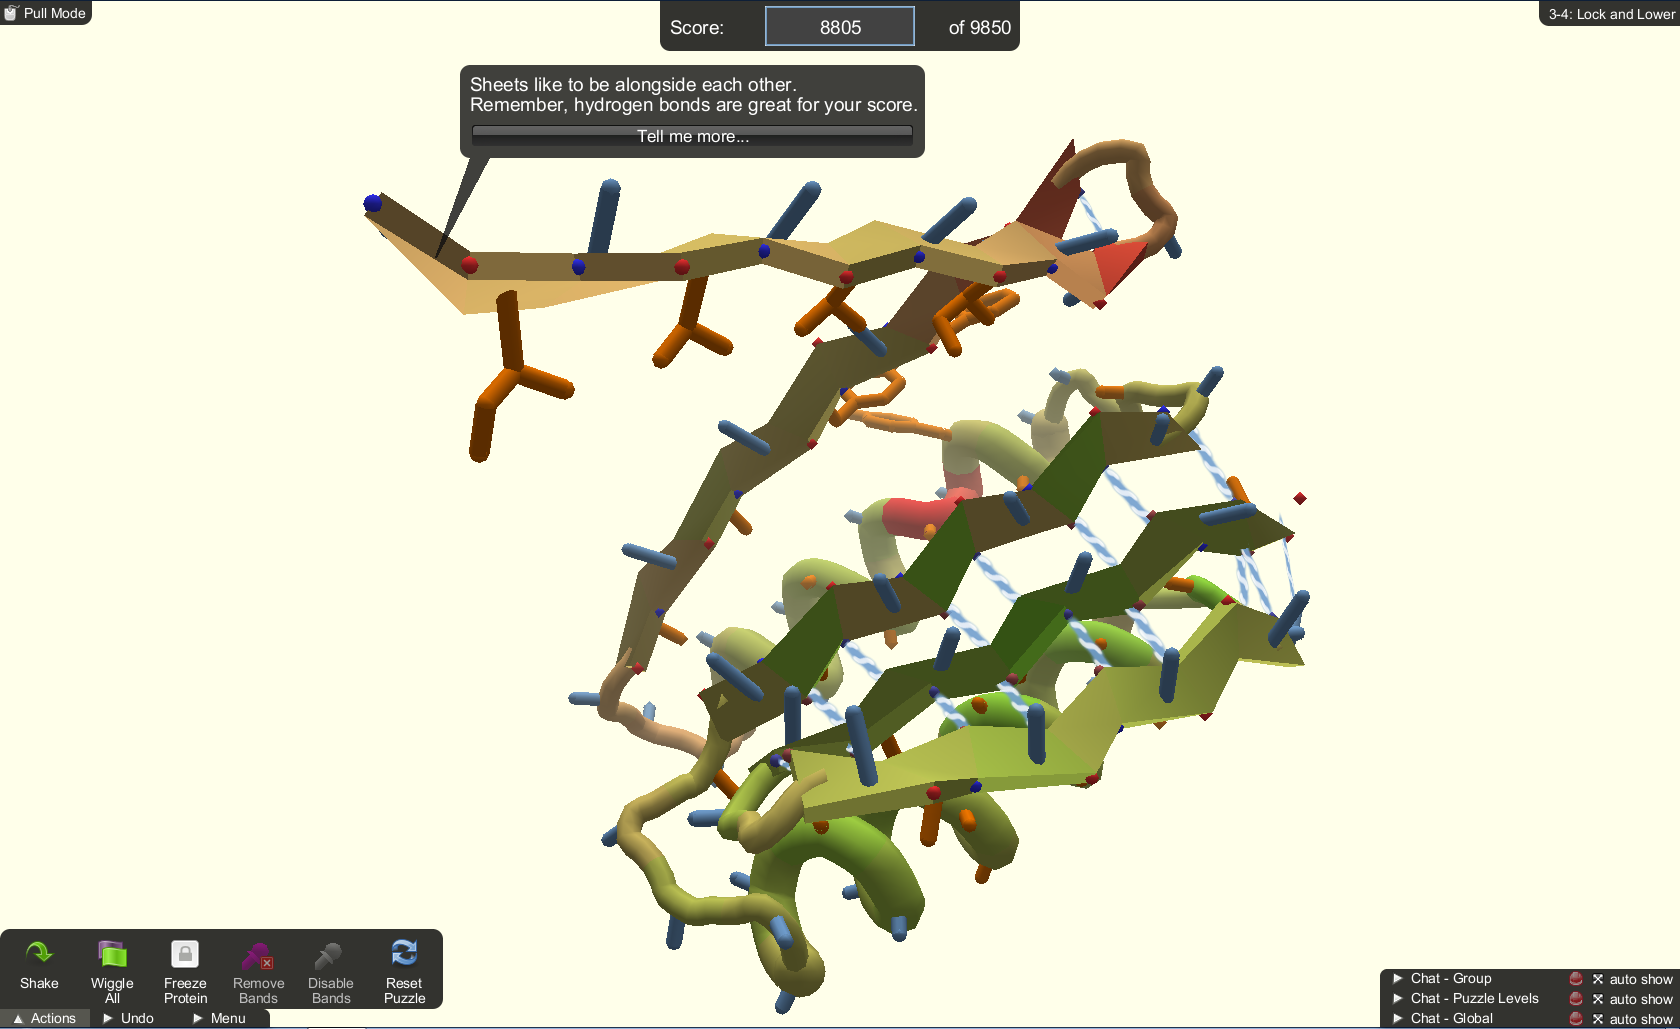
\includegraphics[width=0.8\columnwidth]{foldit.eps}
		\caption{Foldit is solving a serious problem}
		\label{fig:foldit}
\end{figure}

A Serious Alternative Reality Game (ARG) is one type of serious game that blends real and virtual world activities in the serious gaming context. Jane McGonigal designed the award winning serious ARG game ``World Without Oil'' \cite{worldwithoutoil} and ``Evoke'' \cite{urgentevoke} with the goal to empower people to come up with creative solutions to urgent real-world problems. 

ARGs have also been used to support learning. Connolly et al. \cite{connolly2009arguing} discuss the development of an educational ARG to motivate secondary school students across Europe to learn foreign languages. The results of the pilot run of the game in 2009 indicated that 92\% of students felt the game motivated them to learn a second language. One of problems the team identified is the limitation of Moodle platform the game is based on and there is potential to improve the effectiveness of the game.

The report of the ARGOSI project \cite{whitton2009alternate} provides insights into the use of ARGs in game based learning and the challenges they face in the field of higher education. The pilot was run at the University of Bolton with the aim of providing an engaging alternative to traditional methods of introducing students to university life. Adoption of the game was fairly low with 173 players and 23 (13\%) of whom were active. The project identifies a number of questions surrounding educational ARGs, such as motivation, relationship to curriculum, marketing and timing. The report
suggests that a complete ARG model may not be appropriate for wholesale learning, but there is certainly potential in using game elements.

While ``Serious Games'' has been an active research topic for decades, ``Gamification'', on the other hand, is a relatively new subject. Deterding et al. \cite {Deterding2011mt} defines gamification as ``the use of game design elements in non-game contexts''. The term only came into widespread use starting in 2010 \cite {schell2010design} \cite {zichermann2010game}. Gartner \cite {gartnerPress2011} predicts that by 2015, more than half of companies managing innovation processes will employ gamification, applying game mechanics to application areas including productivity, finance, health, sustainability, news, user-generated content and e-learning. 

Deterding et al. \cite{Deterding2011mt} describes the distinctions between gamification, serious games and other related concepts, as shown in Figure \ref{fig:define_gamification}. According to Deterding, a) Gamification is about games. It is different than playful interaction or playful design. b) Gamification uses game elements. It is not a complete game such as a serious game. c) Gamification applies to non-game contexts. Similar to serious games, gamification uses games for other purposes than its normal expected use for entertainment. d) Gamification focuses on design. It is not game-based technology or practice of wider game ecology.

\begin{figure}[htbp]
	\centering
		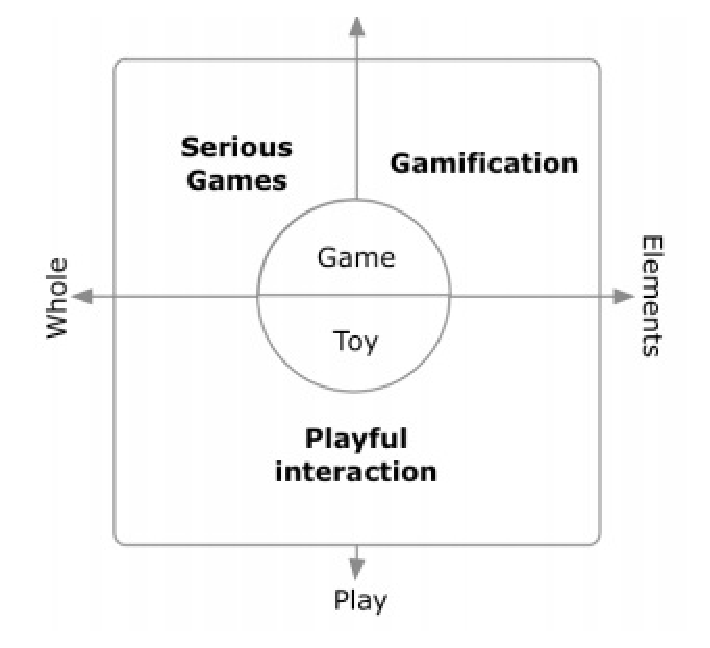
\includegraphics[width=0.5\columnwidth]{defining_gamification.eps}
		\caption{Serious Game and Gamification (source: Deterding \cite{Deterding2011mt})}
		\label{fig:define_gamification}
\end{figure}

While they are different, both gamification and serious games are trying to solve problems with game thinking. Gamification's main driving force is motivation, similarly, serious games also try to solve the motivation problem and influence people's behavior for ``serious'' purpose.  Bosch \cite{bosch2011} considered the serious game Foldit as a successful example of gamification in science.

FourSquare \cite{foursquare} is probably the most recognized example of applying game mechanics to a location based networking application. It is a location based game like service where players check-in to locations for virtual points and rewards.  By employing gamification elements such as points, badges, levels and leader boards, it engages users to revisit a location such as a restaurant or pub and become a loyal customer and finally the ``mayor'' of the place. Certain virtual rewards such as the ``mayor'' of a particular Starbucks can be converted into real products, e.g. a free coffee. Foursqure proved that simple game mechanics can affect user behavior by engaging 10 million customers with a successful business model.

\begin{figure}[htbp]
	\centering
		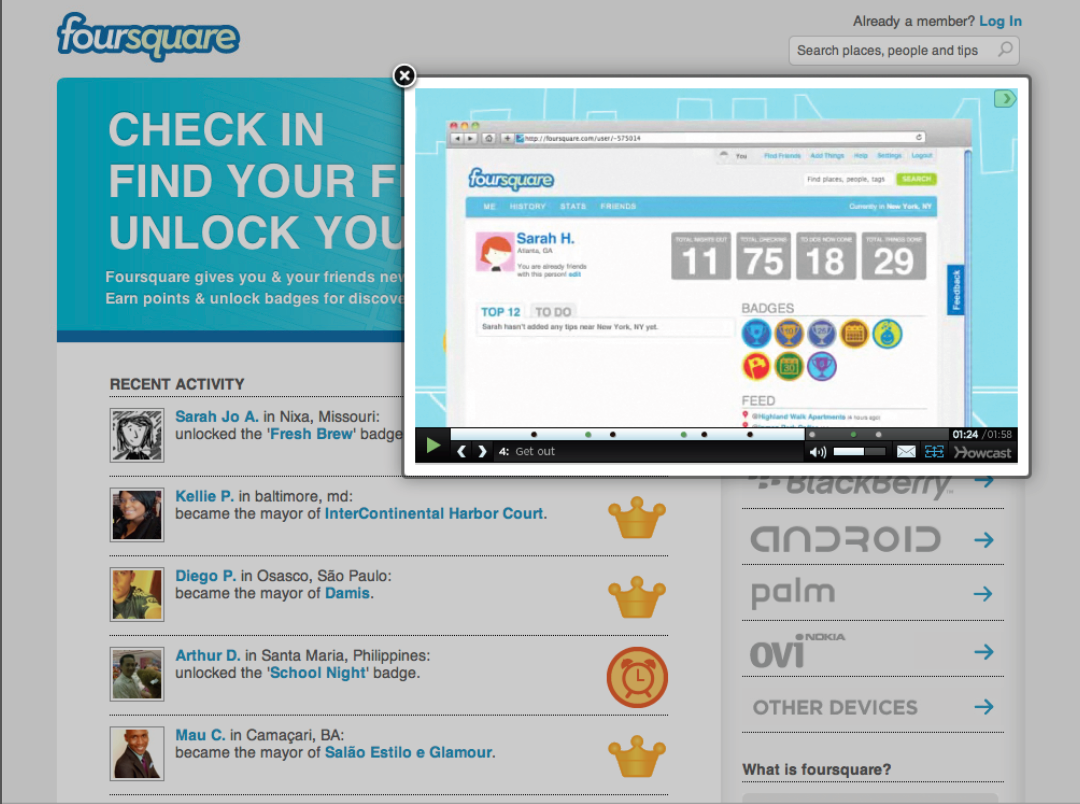
\includegraphics[width=0.7\columnwidth]{foursquare.eps}
		\caption{Foursquare makes modern badges popular}
		\label{fig:foursquare}
\end{figure}

Nike+ \cite{nikeplus} is a social running game that employs game mechanics to encourage runners - both casual and hardcore - to compete and improve their fitness, with the goal of solving the main problem of most fitness programs: motivation. Nike+ allows runners to upload their exercise data to its web site, and start challenging themselves and their friends. They can also get support from their friends through the web site. The game makes running and exercise fun, which eventually serve the ``serious'' purpose of making people healthy.

\begin{figure}[htbp]
	\centering
		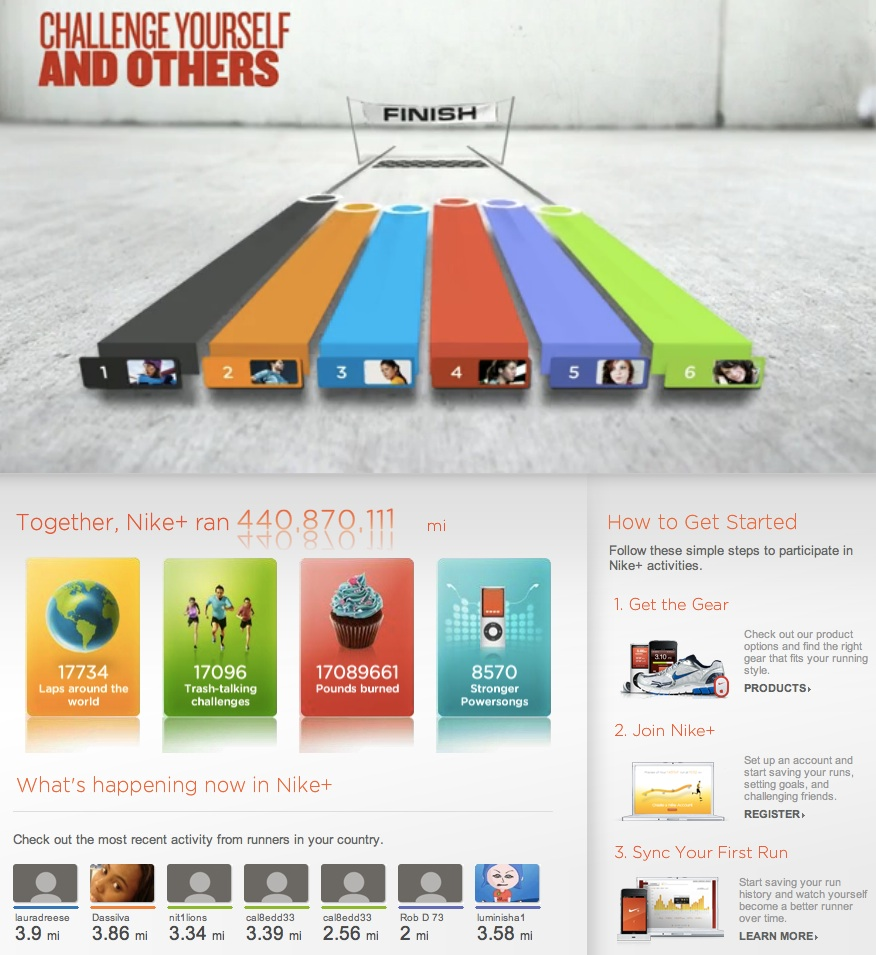
\includegraphics[width=0.6\columnwidth]{nikeplus.eps}
		\caption{Nike+ makes fitness run}
		\label{fig:nikeplus}
\end{figure}

RibbonHero \cite{ribbonhero} is a game that helps users discover new Microsoft Office features. The goal is to have users build familiarity and expose them to the Office UI, so that they understand what kind of features are available. According to the creator of the game, Office ``has a lot of powerful features that users might not know but can be really useful''. The game gives users a chance to learn those features through a game interface, rather than reading the software manuals or watching the typically dry IT training videos.

\begin{figure}[htbp]
	\centering
		\subfigure[Quest to earn points]{\label{fig:Ribbon1}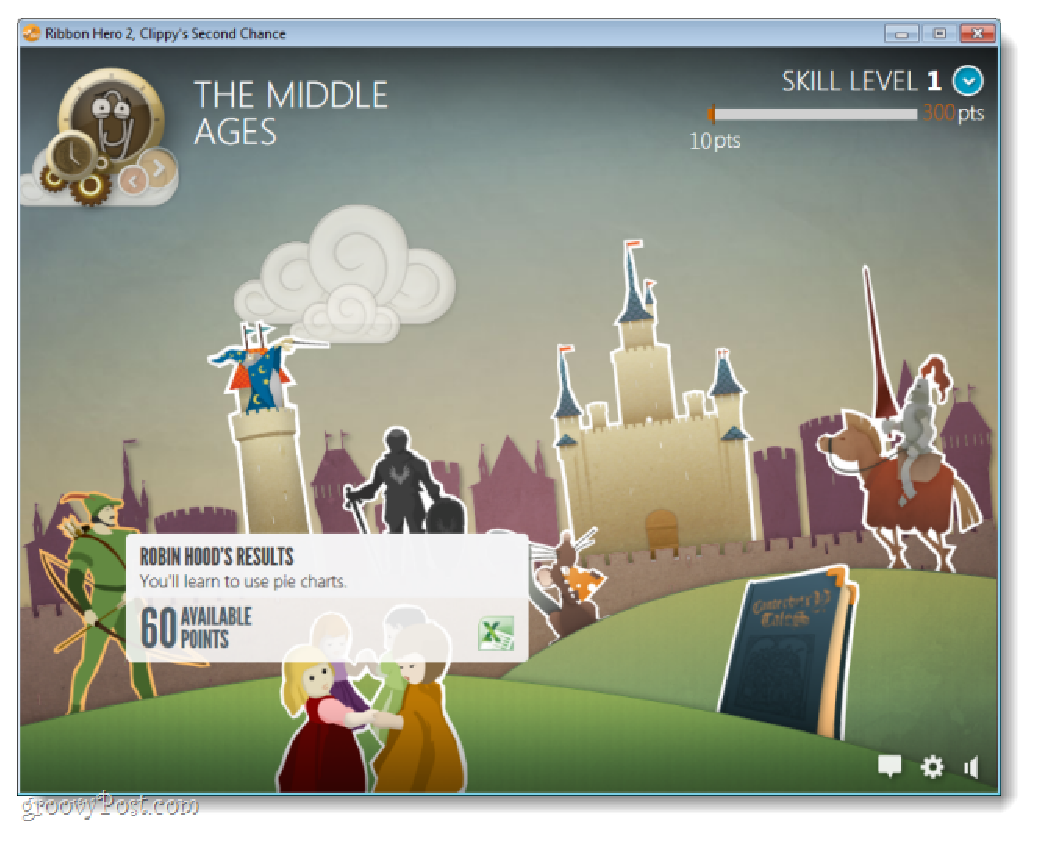
\includegraphics[height=2.5in]{ribbon1.eps}}
		\subfigure[Competing a task]{\label{fig:Ribbon2}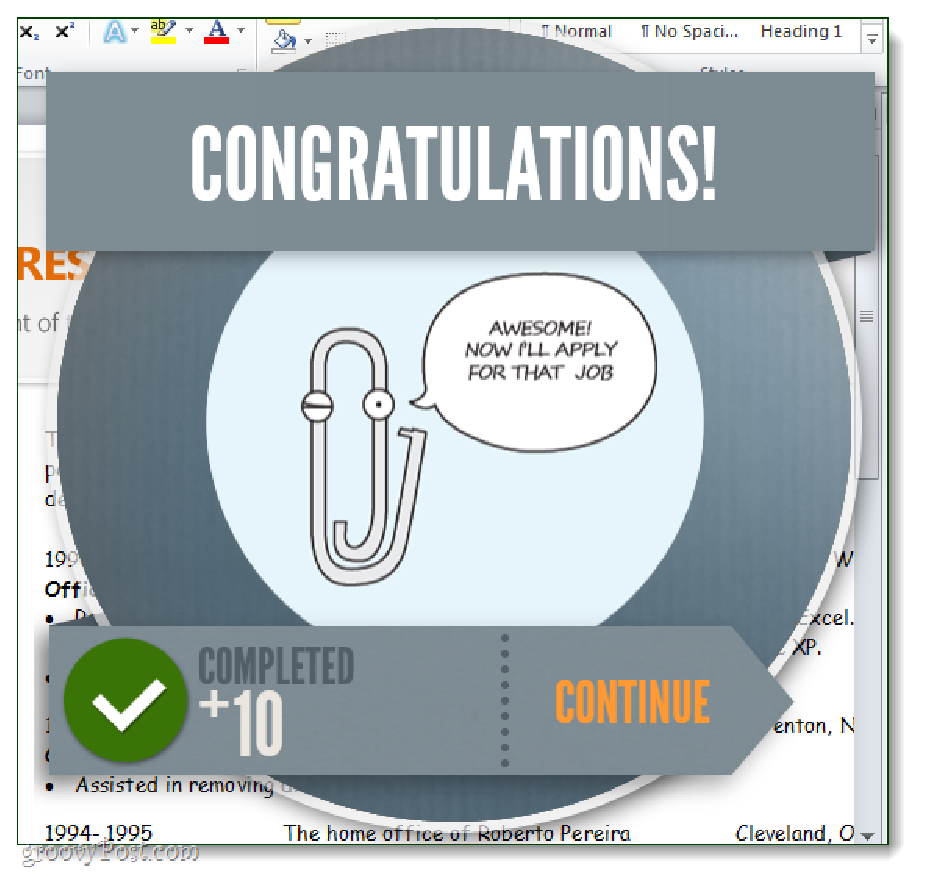
\includegraphics[height=2.5in]{ribbon2.eps}}
		\caption{RibbonHero Helps to Learn Office}
		\label{fig:ribbon}
\end{figure}

Why games? Results of a study published in the May 1998 issue of Nature \cite {koepp1998evidence} demonstrated that video game players experience regular releases of dopamine during game play. Dopamine is a neurotransmitter that signals pleasure rewards for food, sex and addictive drugs, such as cocaine. 

A favorite subject of Greek vase-paintings in the ancient games exhibition in the British Museum's department of Greek and Roman antiquities is Ajax and Achilles playing a kind of board game called backgammon, as illustrated in Figure \ref{fig:ancient-games}. It is noteworthy that both Ajax and Achilles have the full armor on while playing the game. According to Arthur A. Krentz \cite{krentz1998play}, in Plato's ``Republic'', the term ``paideia" (in Greek, means education/culture), ``paidia" (means play/game/pastime/sport), and ``paides" (means children), have the same root. The three terms often show up in the same context. ``The central aim of pedagogy (paidagogia) is to encourage learning as a form of play (paidia), which is the most persuasive and effective approach to learning" .

\begin{figure}[htbp]
	\centering
		
\includegraphics[width=0.4\columnwidth]{roman-game-vase.eps}
		\caption{Ancient Games Shown in British Museum}
		\label{fig:ancient-games}
\end{figure}

Moving forward a couple of millennia, World of Warcraft (WoW) is a massively multiplayer online role-playing game (MMORPG) with 11.1 million subscribers, currently the world's most popular MMORPG.  Nick Yee \cite {yee2002understanding} pointed out that the collaborative nature of most activities makes MMORPG unique. ``It's the people that are addictive, not the game''. ``Most importantly, it is the reward of being socialized into a community of gamers and acquiring a reputation within it''  . He claimed \cite {yee2001vsb} that ``WoW truly is a virtual Skinner box'', smoothly increasing reward and difficulty and reinforcing player commitment along the way.
	
In her popular and inspiring TED talk ``Gaming can make a better world" \cite {mcgonigal2010ted} and in her book ``Reality is Broken" \cite {mcgonigal2011reality}, researcher and game designer Jane McGonigal makes a case for why good games make us better, and how they can help us change the world. She notes that more than 3 billion hours a week is spent in playing video game by our society. She says that the average gamer plays 10,000 hours of games by age 21. That's about the same number of hours that students spend in high school and middle school. There are 500 million gamers today, playing on all sorts of platforms from the iPhone to game consoles. Instead of the common conception that gaming is a waste of time, she argues that ``playing games is the single most productive thing we can do with our time'' and that is  the solution to our ``Broken Reality''. Byron Reeves also argues in his book ``Total Engagement" \cite {reeves2009total}, that games, especially MMO type games, can change the way people work and businesses compete.

Psychology professor Mihaly Czikszentmihalyi introduced a specific kind of happiness that he named ``flow" \cite{csikszentmihalyi1991flow}, which is considered as one of the fundamental reasons that people play games \cite{murphygames}. Flow is a state of absorption, characterized by intense concentration, loss of self-awareness, a feeling of being perfectly challenged (neither bored nor overwhelmed) and a sense that time is flying. In order to achieve flow, the important condition is a balanced goal that is challenging yet achievable within the individual's ability. This balance is referred to as the flow channel as shown in figure 2.7.

\begin{figure}[htbp]
	\centering
		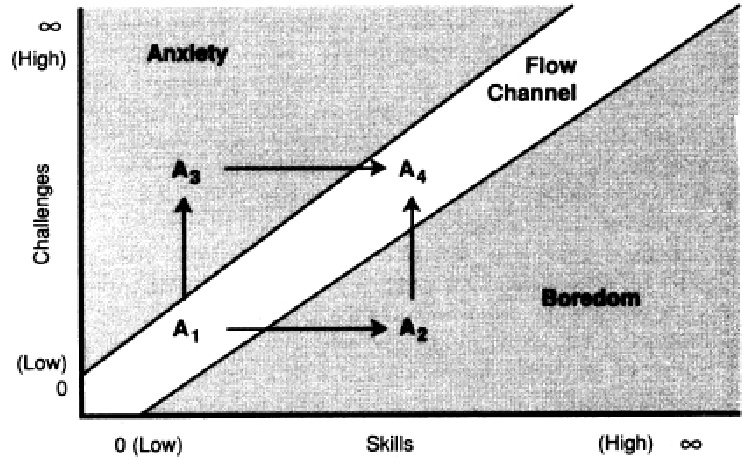
\includegraphics[scale=0.45]{flow.jpg}
		\caption{The state of flow is achieved between anxiety and boredom (source: Czikszentmihalyi \cite{csikszentmihalyi1991flow})}
		\label{fig:state_of_flow}
\end{figure}

In order to understand why people play games, Richard Bartle identified four player personality types by studying players of the Multi-User Dungeon (MUD) game in 1960s \cite {bartle1996hearts}. The four types are based on the 2 underlying axes:

1. Achievers: driven by in-game goals, usually some form of points gathering - whether experience points, levels, or money.

2. Explorers:  driven to find out as much as they can about the virtual construct - including mapping its geography and understanding the game mechanics.

3. Socializers: use the virtual construct to converse and role-play with their fellow gamers.

4. Killers: use the virtual construct to cause distress on other players, and gain satisfaction from inflicting anxiety and pain on others.

Bartle's player type model has been the basic for understanding the player motivation. Dan Dixon presented the limitation and misuse of Bartle's model in general games and gamification contexts \cite{DixonPlayerType}. Amy Jo Kim applied the model in her gamification approach by overlaying social actions from the game on top of the player types \cite {Kim2010}, as shown in Figure 2.8.

\begin{figure}[htbp]
	\centering
		\subfigure[Bartle's Player Types (1996)]{\label{fig:player-types}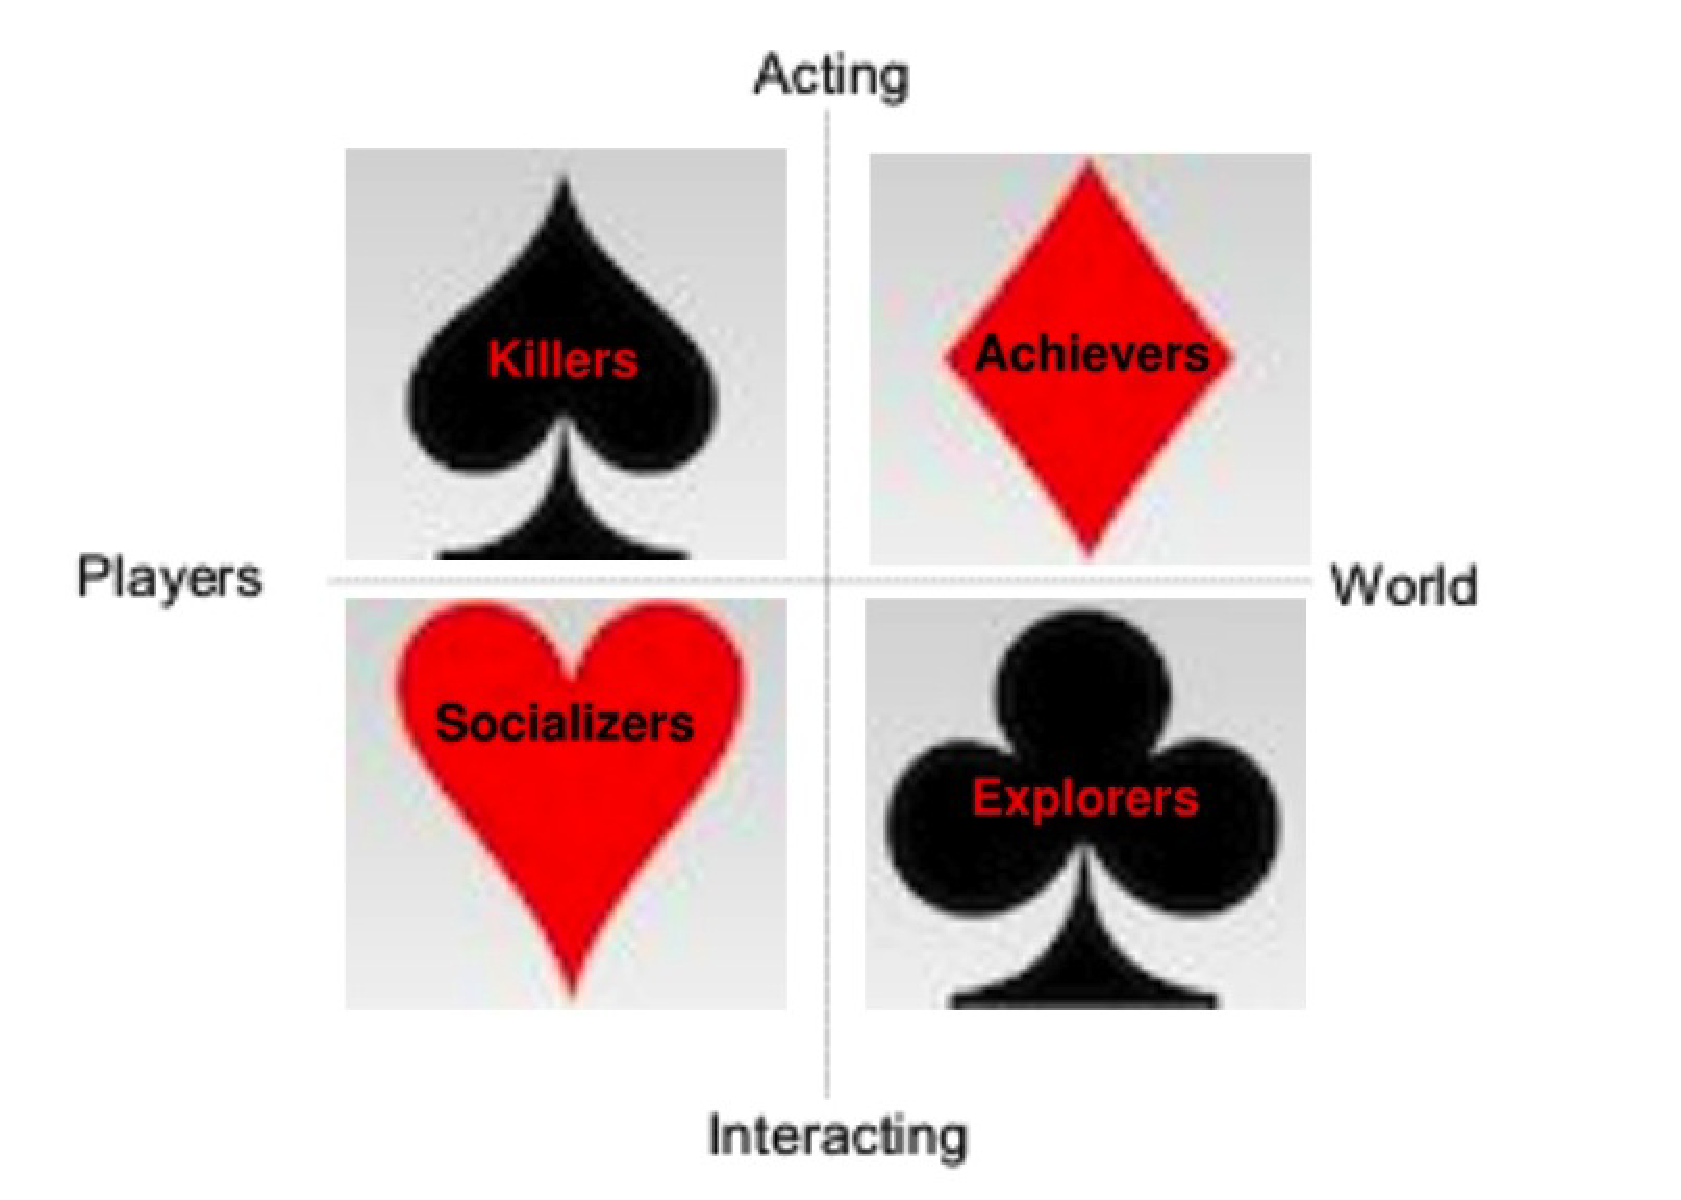
\includegraphics[height=2.0in]{bartle-player-types.eps}}
		\subfigure[Kim's Social Actions (2010)]{\label{fig:social-action}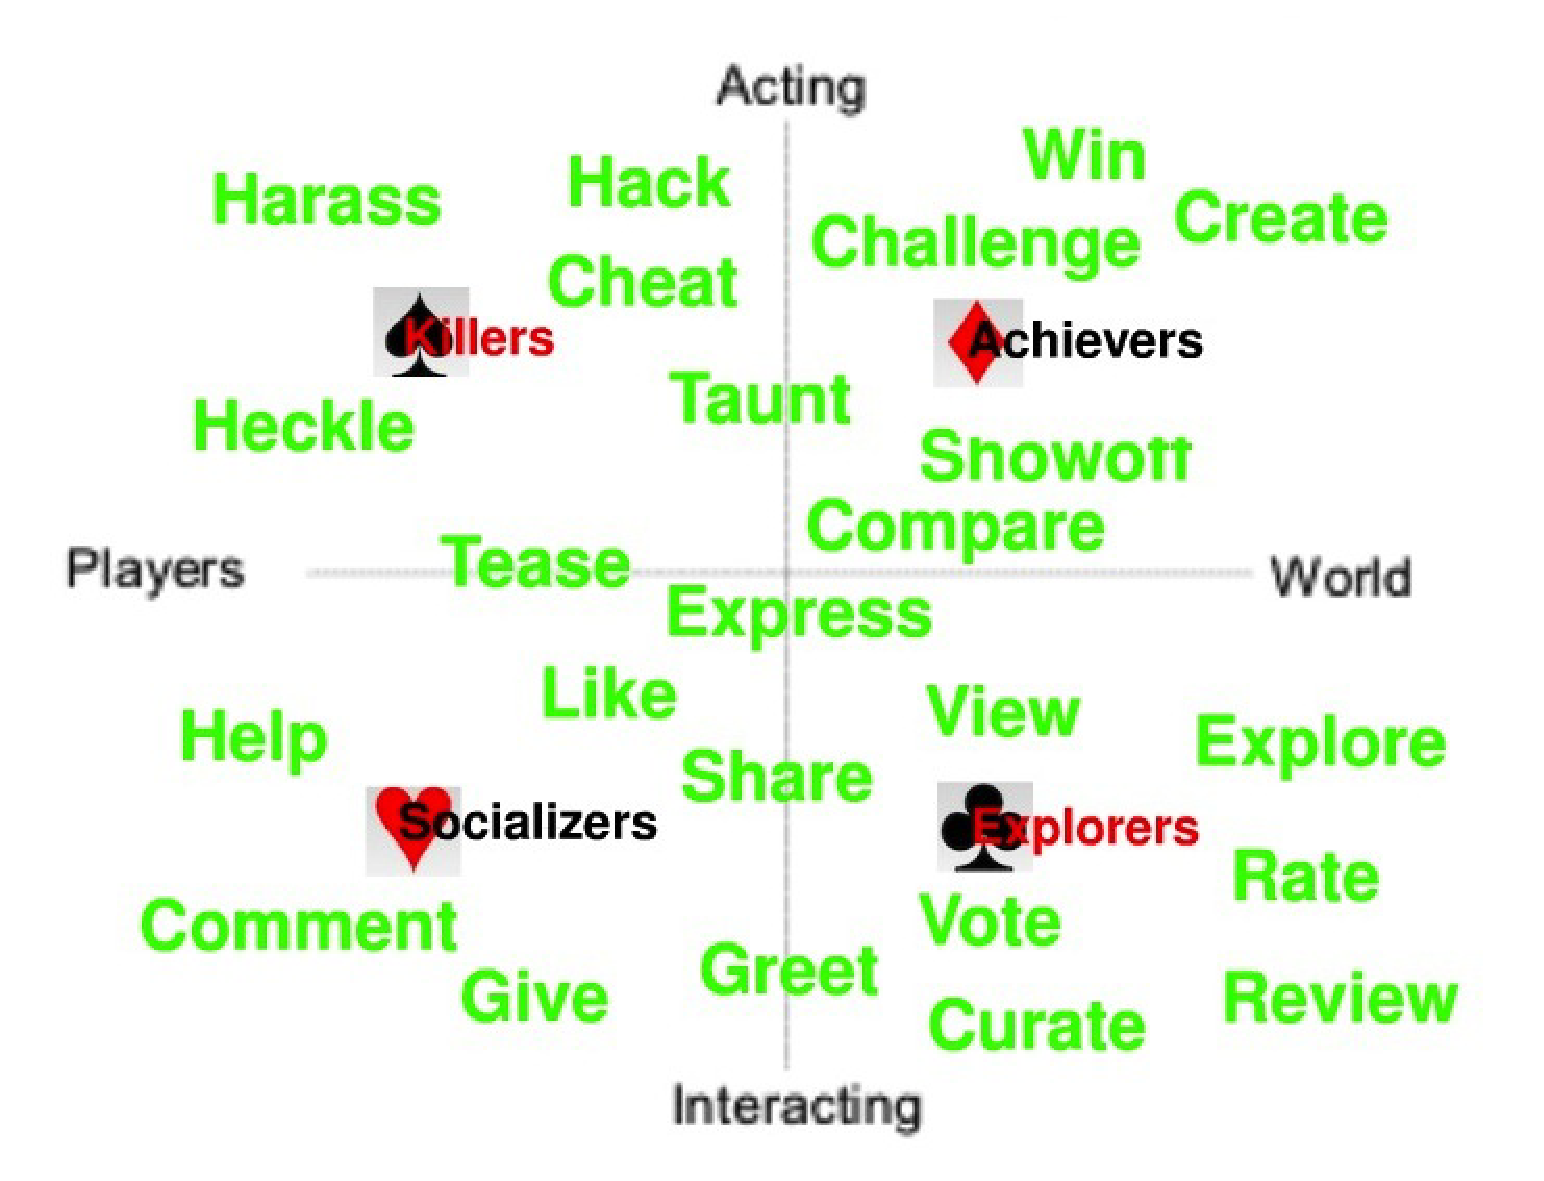
\includegraphics[height=2.0in]{kim-player-types.eps}}
		\caption{Player Types}
		\label{fig:play-types}
\end{figure}

Different game mechanics and elements can be used to serve different functions in satisfying players' needs, and the basic elements such as points, badges, and leader boards are the defining attributes of the current gamification practices \cite {Deterding2011dragon}. \autoref{fig:basic-game-elements}  illustrates these basic game mechanics and elements.

\begin{figure}[htbp]
	\centering
		\subfigure[Satisfies Human Needs (source: Bunchball)]{\label{fig:human-needs}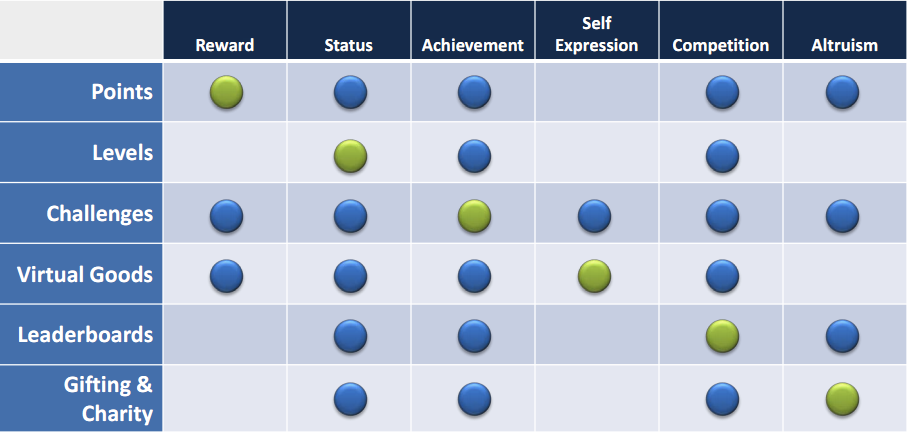
\includegraphics[width=3.2in]{human-needs.png}}
		\subfigure[Basic Mechanics (source: Deterding \cite{Deterding2011meaningful})]{\label{fig:basic-elements (source: }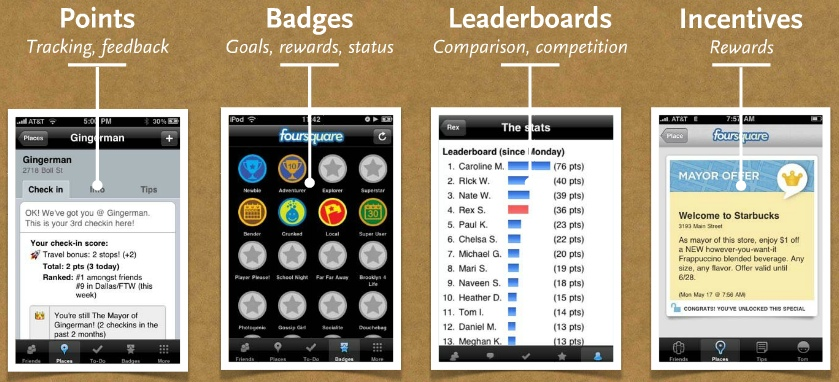
\includegraphics[width=3.2in]{basic-element.jpg}}
		\caption{Basic game mechanics and elements}
		\label{fig:basic-game-elements}
\end{figure}

Seth Priebatsch \cite {Priebatsch2010ted} states that you can get anyone to do anything with 7 game dynamics. Techcrunch \cite{Biggs2010} published a ``secret'' game dynamics play deck that is used by Priebatsch's company SCVNGR. The play deck is a set of 47 flash cards. Each card illustrates one game dynamics. SCVNGR employees are instructed to memorize them and apply in their applications as needed.  Social interaction designer Adrian Chan  \cite {Chan2010} commented that the play deck does not include the sociological factors in social gaming and confuses game mechanics with game dynamics. 

There are many debates and criticism over whether gamification itself is inherently good or bad. 
Many considered the current efforts of gamification focus on extrinsic motivators (such as points, badges and rewards) instead of intrinsic motivators generated by an individual's internal will or desires.

Designer Stephen Anderson claimed that \cite {anderson2011} gamification mistakes extrinsic rewards (rather than intrinsic motivation) for the power of games and hence offers only feedback, not goals \& rules. 

\begin{figure}[htbp]
	\centering
		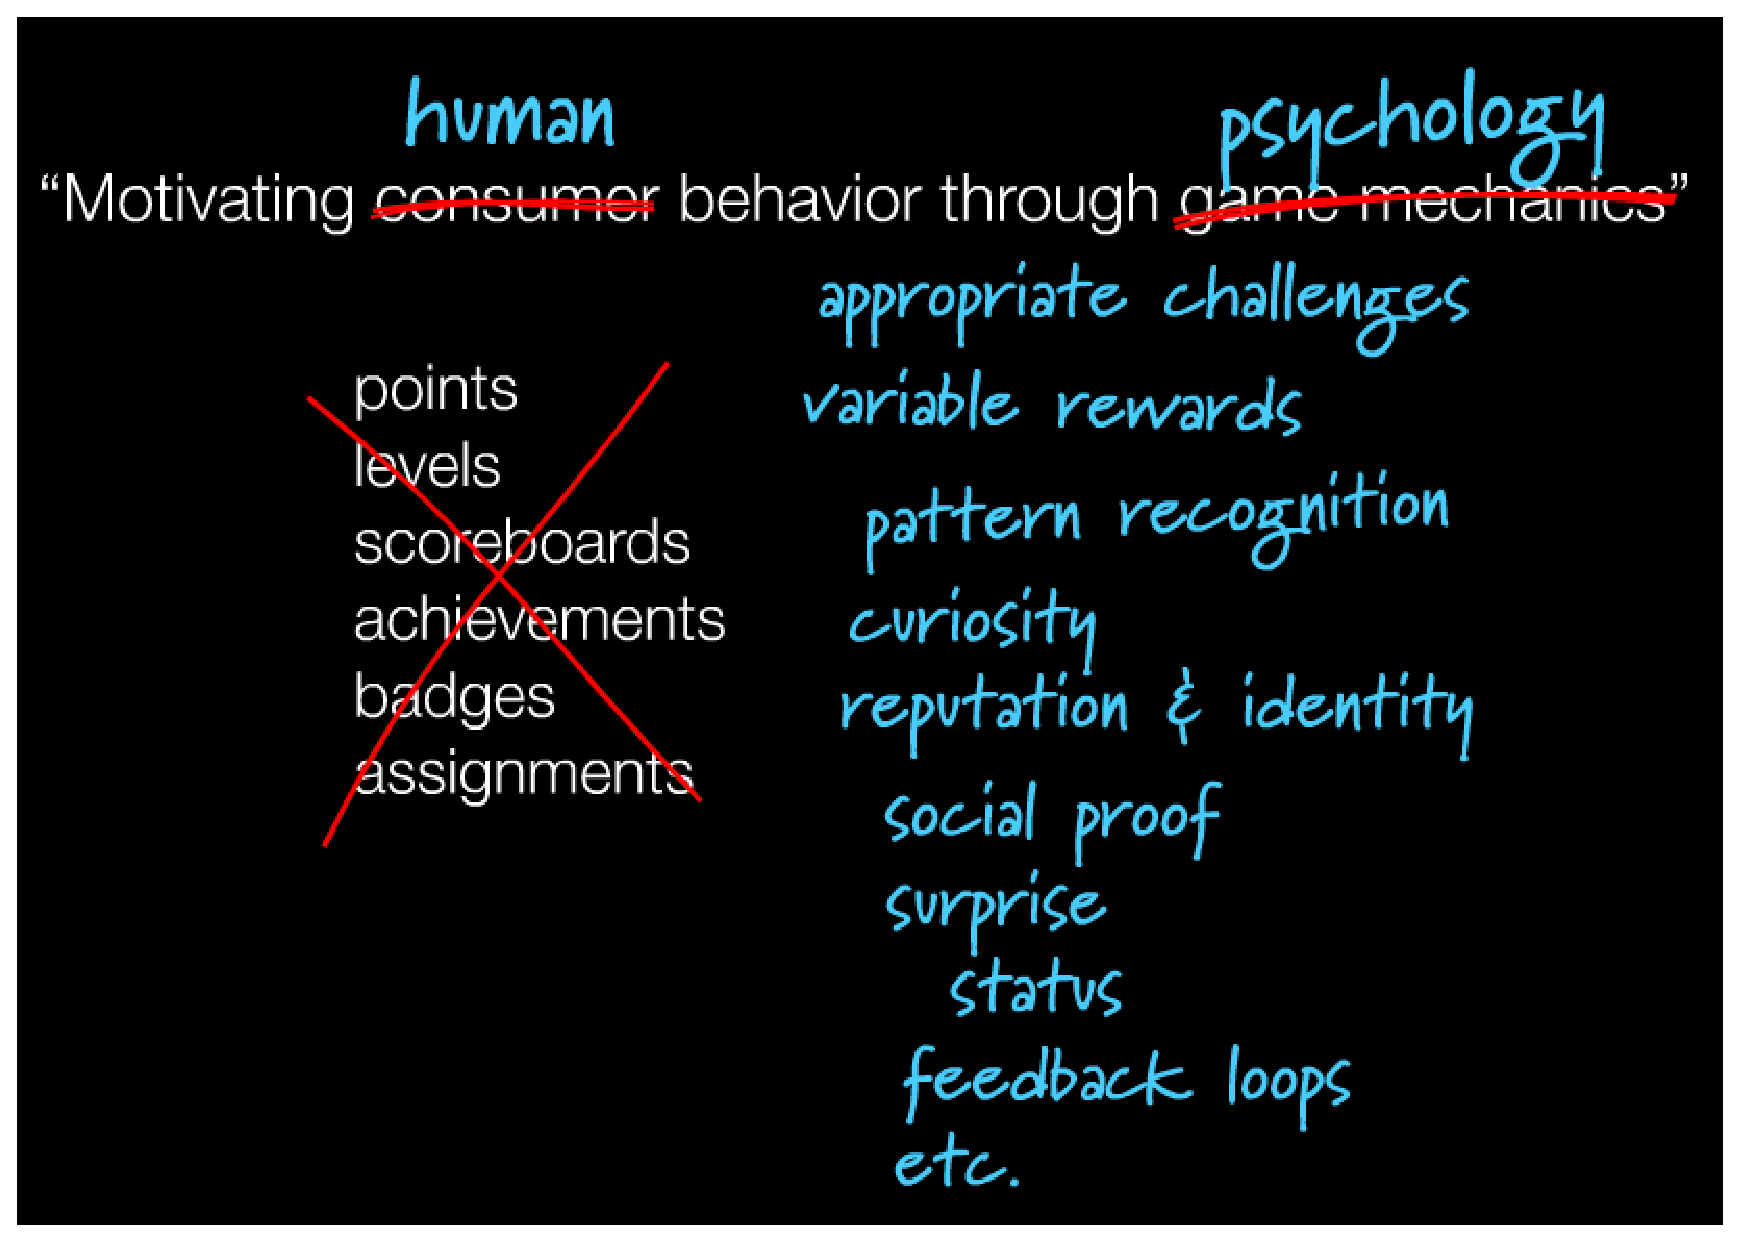
\includegraphics[scale=0.25]{anti-gamification.eps}
		\caption{Gamification is about extrinsic rewards (source: Anderson \cite {anderson2011})}
		\label{fig:anti-gamification}
\end{figure}

Jane McGonigal spoke about her concern about current state of gamification in the GDC 2011 talk titled ``We don't need no stinking badges: How to reinvent reality without gamification'' \cite {mcgonigal2011}. She argued that current gamification confuses intrinsic/extrinsic motivation and proposed ``Gameful Design'' instead of ``Gamification''. She claimed that "Gameful is player-oriented", which presumed that the loyalty program type gamification is product or service oriented. While the current gamification is about extrinsic reward, with points, badges, and levels, gameful design is about intrinsic reward, with positive emotion, relationships, meaning and accomplishment.

Nicole Lazzaro argued that the use of extrinsic rewards will decrease the motivation to use your products and services once you remove that reward \cite {Lazzaro2011}. Vockell resonated that in education psychology, extrinsic motivators may lead to short-range activity increase but reduction in long-range interest in a topic. While intrinsic motivators motivate people best when they are working toward personally meaningful goals \cite{vockell2004educational}. 

Michael Wu argues that extrinsic rewards can jumpstart intrinsic motivation  \cite {WuSustainable2011}. He claimed that gamification just has to work long enough for some other processes to take over as the primary driver of value. Subsequently, it becomes a secondary reinforcement system. 

In order to design a game that that is intrinsic motivated, Amy Jo Kim presented ``Smart Gamification'' which focuses on designing an effective ``Player Journey'' with intrinsic reward preferred over extrinsic reward \cite {Kim2010}. Kim pointed out that game techniques are not equal to core experience and intrinsic values are greater than extrinsic rewards. Kim stated that ``a good game take the player on a journey toward mastery". As illustrated in \autoref{fig:player-lifecycle}, when over time players progress from newcomer to regular and finally to enthusiast, they progress from novice to expert to master. Kim also incorporates the MDA framework \cite {hunicke2004mda} by using it to guide and motivate the player journey as illustrated in \autoref{fig:game-design}.

\begin{figure}[htbp]
	\centering
		\subfigure[Player Lifecycle]{\label{fig:player-lifecycle}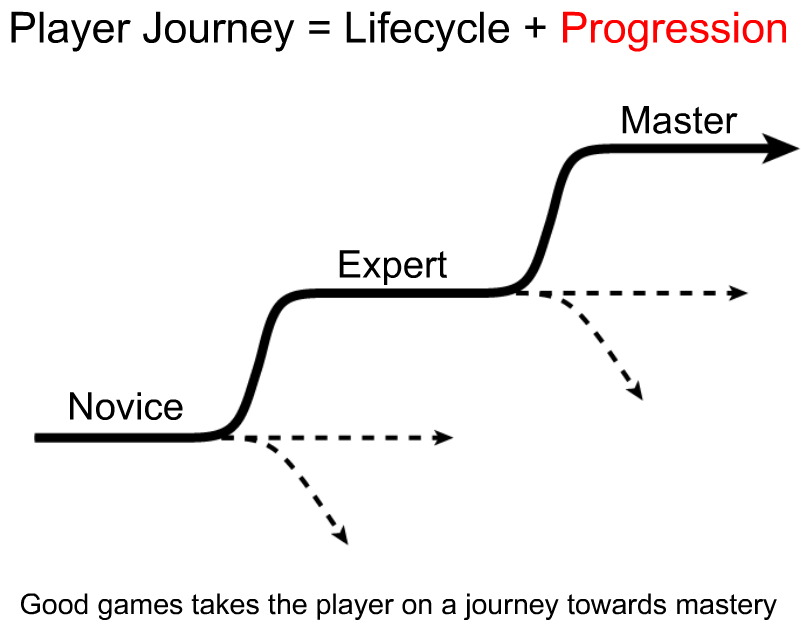
\includegraphics[height=2in]{kim-workshop.png}}
		\subfigure[Game Design]{\label{fig:game-design}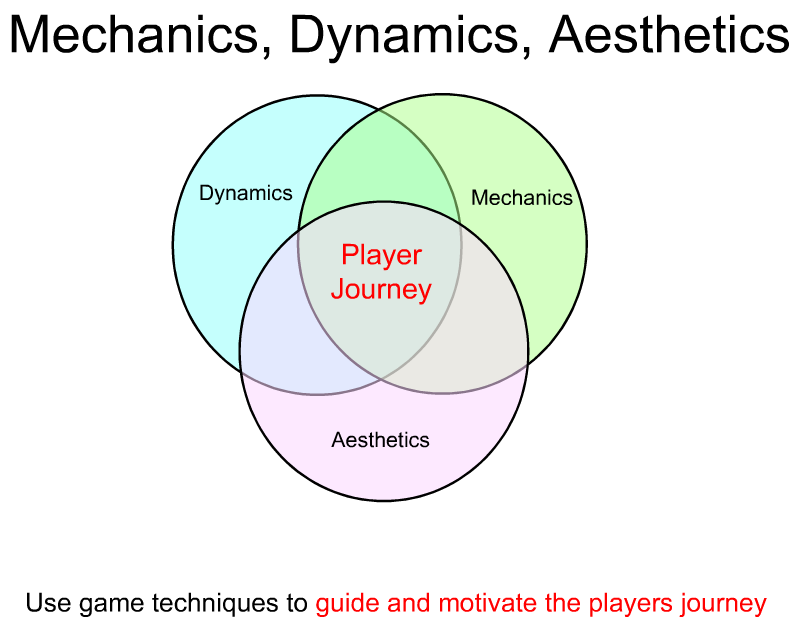
\includegraphics[height=2in]{kim-workshop2.png}}
		\caption{Designing Player Journey (source: Kim \cite {Kim2010})}
		\label{fig:design-player-journey}
\end{figure}

Similarly, researcher Sebastian Deterding not only criticized the current practice of simple gamification practices but stressed the important of ``meaningful play'' and proposed a user experience design around the three most important aspects: Meaning, Master and Autonomy \cite {Deterding2011meaningful}. It is an adaptation to the three elements to motivate people in Daniel Pink's book ``Drive: The Surprising Truth About What Motivates Us" \cite {pink2009drive}. Deterding explained that the reason why we play is because of the meaning and autonomy with choice in the game. The mastery in the game give us fun and enjoyment.

\section{Serious Games for Sustainability}
\label{sec:rel-sg-sustainability}

Serious games for sustainability are games designed to achieve the goal of sustainability development.  Reeves et al. \cite{Reeves2011powerhouse} described the design of Power House, an energy game that connects home smart meters to an online multiple player game with the goal of improving home energy behavior. In the game, real world energy data is transformed into a ``more palatable and relevant form of
feedback'', and players may be incentivized by the in-game rewards to complete more energy-friendly real-world behaviors.

\begin{figure}[htbp]
	\centering
		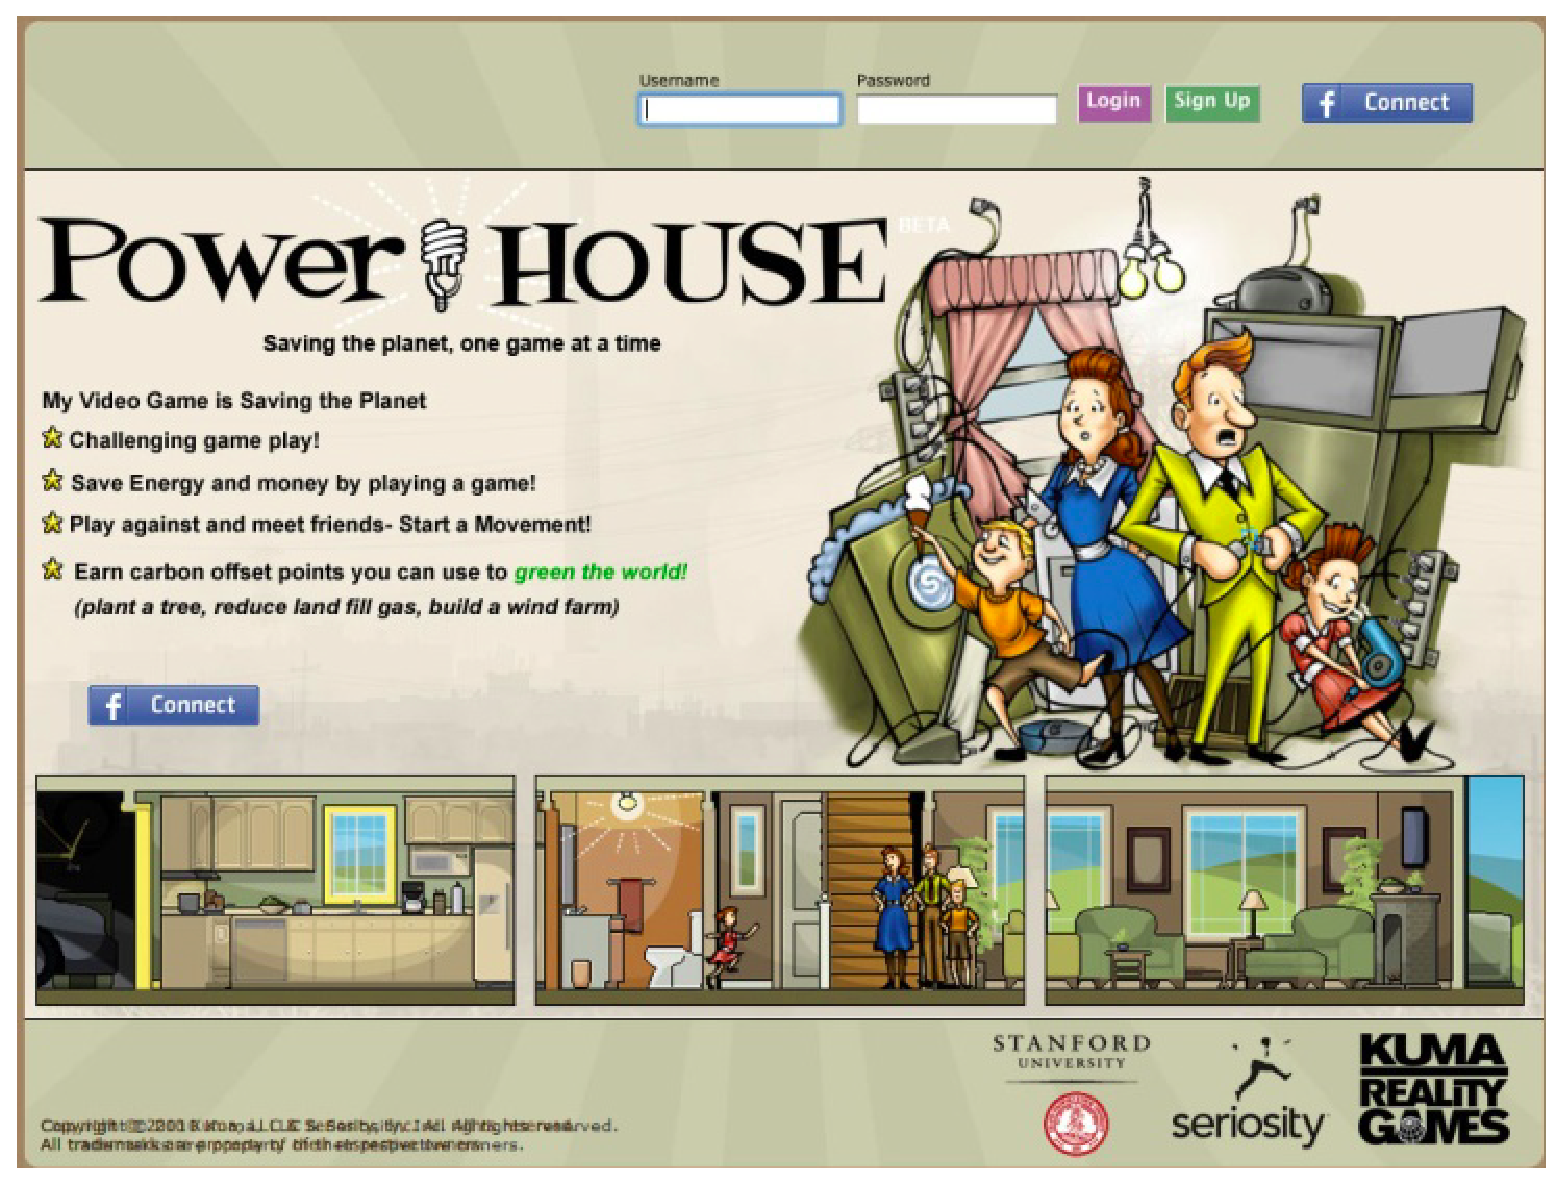
\includegraphics[width=0.8\columnwidth]{powerhouse.eps}
		\caption{Power House Game to Save Energy(source: Reeves \cite{Reeves2011powerhouse})}
		\label{fig:powerhouse}
\end{figure}

RecycleBank \cite {recyclebank} introduced a series of ``Green Challenges'' that used gaming techniques online to motivate participants to learn about green living and to take small green actions to live more sustainable lives offline. According to this report \cite {gamingforgood}, 49,000 individuals participated in the ``Green Your Home Challenges''. Partnered with Google Analytics and ROI research, they found that:
\begin{itemize}
	\item Gamification can increase awareness of positive environmental actions. 97\% of participants surveyed said the game increased their knowledge of the environment.
	\item Games can drive individuals to take positive social and environmental actions. Most participants surveyed indicated they are very or extremely likely to take green actions as a result of participating in the challenge.
	\item Games are an effective and appealing educational tool. 86\% participants agreed online games and contest can be a good way to inform and educate them personally.
\end{itemize}

\begin{figure}[htbp]
	\centering
		\subfigure[Green Your Home Challenge]{\label{fig:RecycleBank1}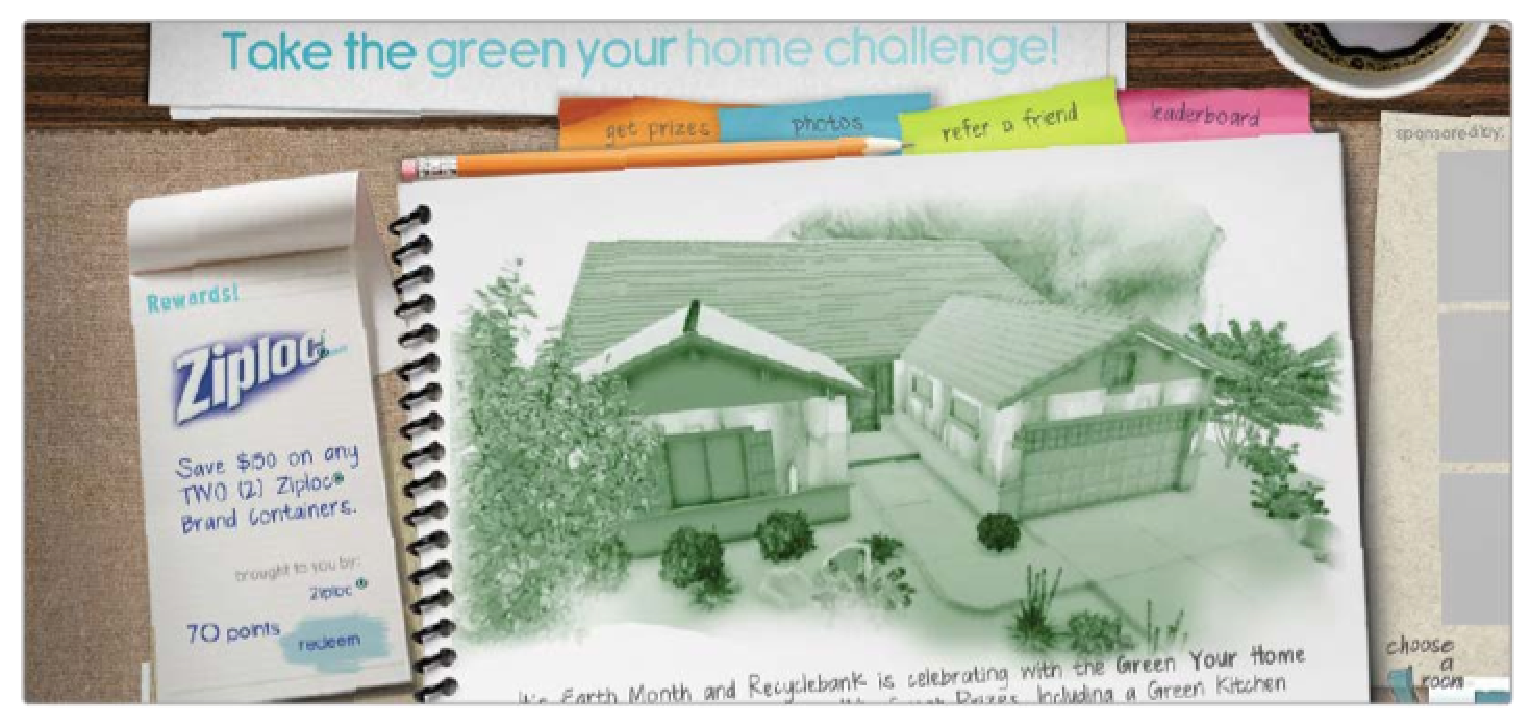
\includegraphics[width=0.7\columnwidth]{recyclebank1.eps}}
		\subfigure[Game Change Behavior]{\label{fig:RecylceBank2}
\includegraphics[width=0.7\columnwidth]{recyclebank2.eps}}
		\caption{RecycleBank - Gaming for Good}
		\label{fig:recyclebank}
\end{figure}

Interactive design also applies game elements in their design to achieve sustainability goal. One example is the ``SmartGauge'' dashboard \cite {ideo2009} for Ford's hybrid cars, where a digital plant responds to how energy-efficient the users driving behavior is. The design gives drivers a game, with the goal to grow more lush and beautiful leaves, a visual reward, by driving efficiently and thus promotes a more environmental behavior. Similarly, The design of ``Piano Staircase'' \cite {funtheory2009}, created by Volkswagen Sweden, installed in a metro station in Stockholm, is to make the staircase next to the escalator look and respond like a piano keyboard, so that every step on the stair will generate different piano sounds every time a commuter walked on it. Observation indicates that 66 percent more people chose to play the ``piano staircase'' game over using the escalator. It is a good example of gameful design for persuading and encouraging energy-efficient behavior.

 \begin{figure}[htbp]
	\centering
		\subfigure[Efficiency Leaves]{\label{ixd-dashbard}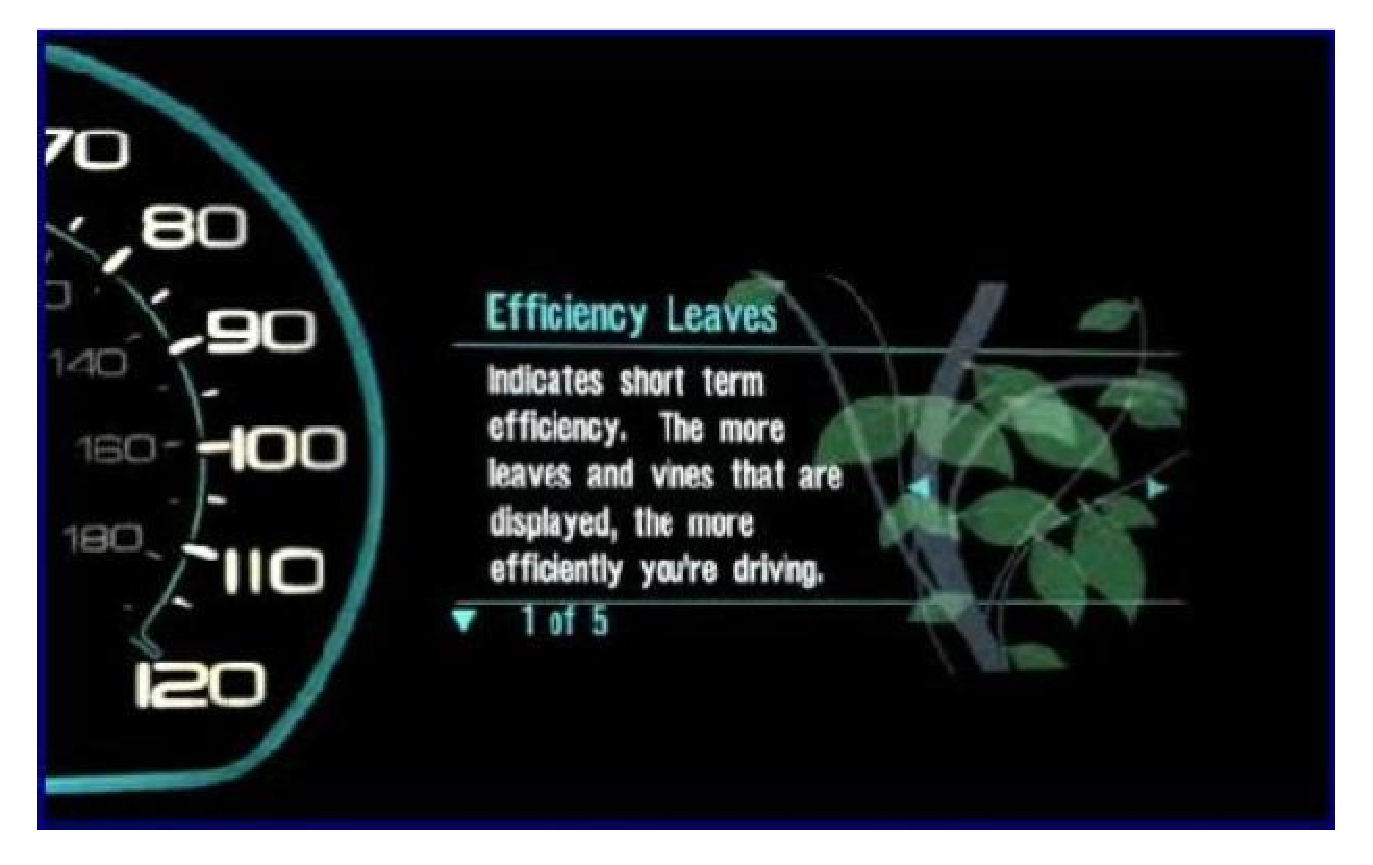
\includegraphics[width=0.7\columnwidth]{ixd-dashboard.eps}}
		\subfigure[Piano Stair vs. Escalator]{\label{fig:ixd-pianostair}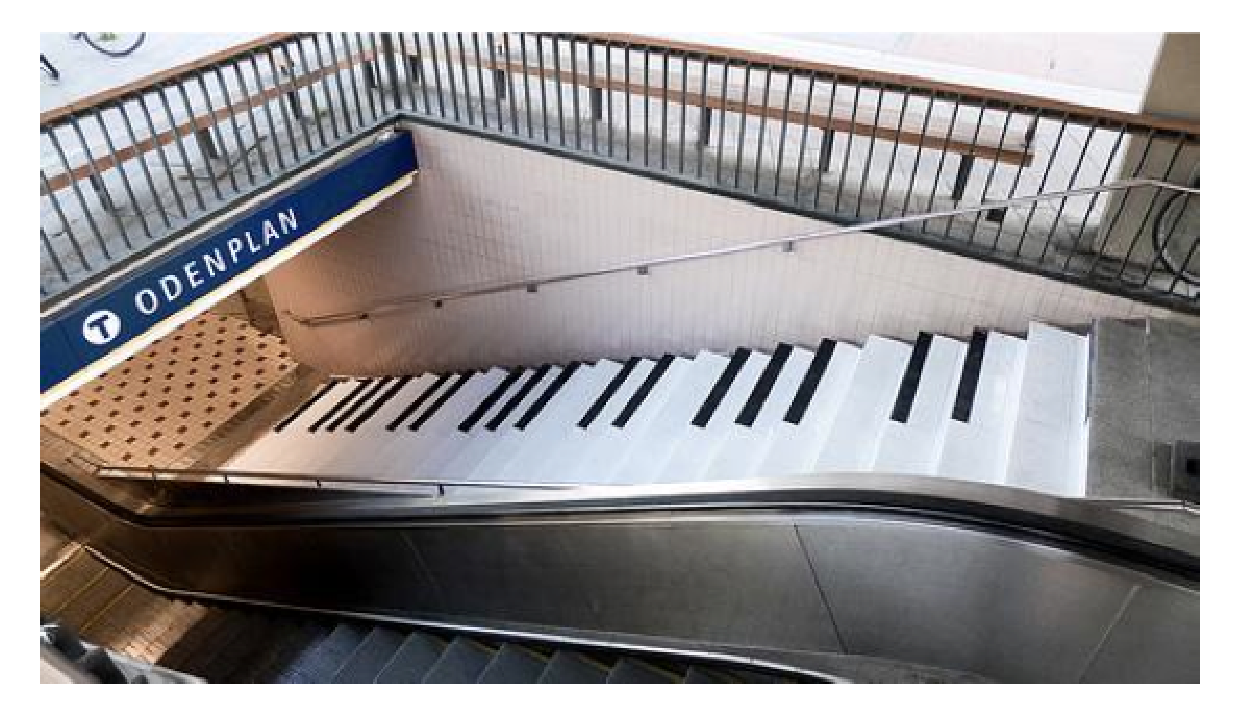
\includegraphics[width=0.7\columnwidth]{ixd-pianostair.eps}}
		\caption{Gameful Design for Sustainability}
		\label{fig:ixd}
\end{figure}	

Energy competitions or challenges have been introduced to college dormitories and residential homes as ways to facilitate and incentivize energy reduction. Petersen et al. \cite{petersen-dorm-energy-reduction} describe their experiences deploying a real-time feedback system in an Oberlin College dorm energy competition in 2005 that includes 22 dormitories over a 2-week period. They found a 32\% reduction in electricity use across all dormitories. However, in a post-competition survey, respondents indicated that some behaviors, such as turning off hallway lights at night and unplugging vending machines were not sustainable outside the competition period.  There has been little analysis on energy usage after the competitions finish, or how positive behavior changes could be sustained.

\begin{figure}[htbp]
	\centering
		
\includegraphics[width=0.7\columnwidth]{oberlin.eps}
		\caption{Energy Competition for Sustainability}
		\label{fig:oberlin}
\end{figure}

-------
Energy competitions are becoming increasingly prevalent across the United States.
Chelsea Hodge found that 163 universities and colleges held or planned to hold an energy competition
during the 2010-2011 academic year [13]. Furthermore, 40\% of these organizations are holding
a competition for the first time. Hodge also found that these competitions are successful, with the
top 25\% of universities reducing energy usage within a building by 12% on average.

on an iPhone.
Despite these shortcomings, Lucid Design Group�s Building Dashboard has become a
very popular option. Lucid�s latest project is the Campus Conservation Nationals [35], a sustainability
competition involving multiple colleges and universities across the United States and Canada.
Their pilot competition had over 40 participants and was held in November 2010. They succeeded
in reducing energy usage by 508,000 kilowatt-hours and water usage by 730,000 gallons. Their next
competition will be in 2012, where they have over 170 colleges and universities signed up.
---------

\section{Serious Game Frameworks}
\label{sec:rel-sg-framework}

Game frameworks (also known as game engines) \cite{sherrod2006ultimate} are ``comprised of a collection of different tools, utilities, and interfaces that hide the low-level details of the various tasks that make up a game''. Examples of game frameworks include:
\begin {itemize}
    \item Unreal \cite{unrealengine}:  The Unreal Engine is a game engine developed by Epic Games, it is primarily used in first person shooter games, providing tools and building blocks for 3D rendering, collision detection, AI, networking etc.
    \item PapayaMobile \cite{papayamobile}: PapayaMobile is a free cross platform social game engine on Android and iOS platform. It provides an SDK and a platform for mobile game developers to create and release games in a ``user-friendly, straightforward way''.
    \item OpenLabyrinth \cite{openlabyrinth}: OpenLabyrinth is an open source game framework that allows its users to create, run and analyze a wide range of different pathway-based activities for healthcare education.
    \item Fabula \cite{fabula}: Fabula is an open source Python game engine for adventure, role-playing and strategy games and digital interactive storytelling. It provides a library and game world abstraction intuitive to people who have not been involved in game development before and hide as much as low level technical details as much as possible.
\end {itemize}

One of the benefits of using a game framework is that, if correctly designed, it will provide useful and reusable ``building blocks'' with which to develop a variety of games. Similarly, serious game frameworks also provide building blocks that enable the serious game developer to focus more time and thought on content and results instead of on the technical details and infrastructure for creating the serious game.

There are two serious game frameworks related to sustainability development. One such framework is the Building Dashboard \cite{building-dashboard}, developed by Lucid Design Group, as shown in Figure \ref{fig:building-dashboard}.

\begin{figure}[htbp]
	\centering
		
\includegraphics[width=0.6\columnwidth]{building-dashboard.eps}
		\caption{Building Dashboard (source: Lucid \cite{building-dashboard})}
		\label{fig:building-dashboard}
\end{figure}

Building Dashboard is commercial platform that ``enables energy reduction competition and empowers building occupants to become active participants in energy management''. It is used to support the Campus Conservation Nationals (CCN) \cite{competetoreduce}, a nationwide electricity and water use reduction competition on college campuses. In CCN 2014, the framework was used by 109 schools in North America to display the energy and water consumption of the competition participants. It enables viewing, comparing and sharing building energy
and water use information on the web through a visual interface, but the
cost of the commercial system creates a barrier to wider adoption. In addition, the
Building Dashboard solution focuses on providing energy information as
a passive media. Besides a scoreboard, there is little interaction between participants
and the system.

Another framework related to sustainability is the Stanford Energy Services Platform \cite{Armel-2012}, as shown in Figure \ref{fig:stanford-platform}. It provides services to support the creations of energy efficiency program and research. The services include data storage, a recommendation system, user registration and participation assignment, surveys and analytics. It had been utilized to support
the implementation of several of Stanford's energy saving projects and energy related serious games, such as the Power House game, Power Down game, and Energy Calculator. At this point, there is not enough information about the Stanford Energy Services Platform regarding the availability and features. 

\begin{figure}[htbp]
	\centering
		
\includegraphics[width=0.6\columnwidth]{stanford-esp.eps}
		\caption{Stanford Energy Services Platform (source: Stanford \cite{Armel-2012})}
		\label{fig:stanford-platform}
\end{figure}
 
%% TODO: add non-serious game framework assessment
\section{Serious Game Framework Assessment}
\label{sec:rel-sg-assessment}

This section examines the assessment of serious game frameworks. It starts by  looking at the assessment of serious games, then looks at the assessment of game frameworks in general, finally examines the assessment of serious game frameworks in particular.

One fundamental question in evaluating a serious game is the extent to which the
game achieves its ``serious'' purpose.  This is quite different from 
traditional entertainment games, in which evaluation focuses on usability or
playability \cite{song2007new}. In the field of serious games, there is an increasing
focus on the methodology of game evaluation \cite{Mayer2012233}. 

De Freitas and Oliver \cite{de2006can} point out that there are few frameworks to support the evaluation of education games. They introduce a four dimensional framework for evaluating 
educational games and simulations. The framework consists of: the context, the pedagogy, the representation, and the learner (or player). Figure \ref{fig:four-dimensional-framework} illustrates the evaluation framework.

\begin{figure}[htbp]
	\centering
		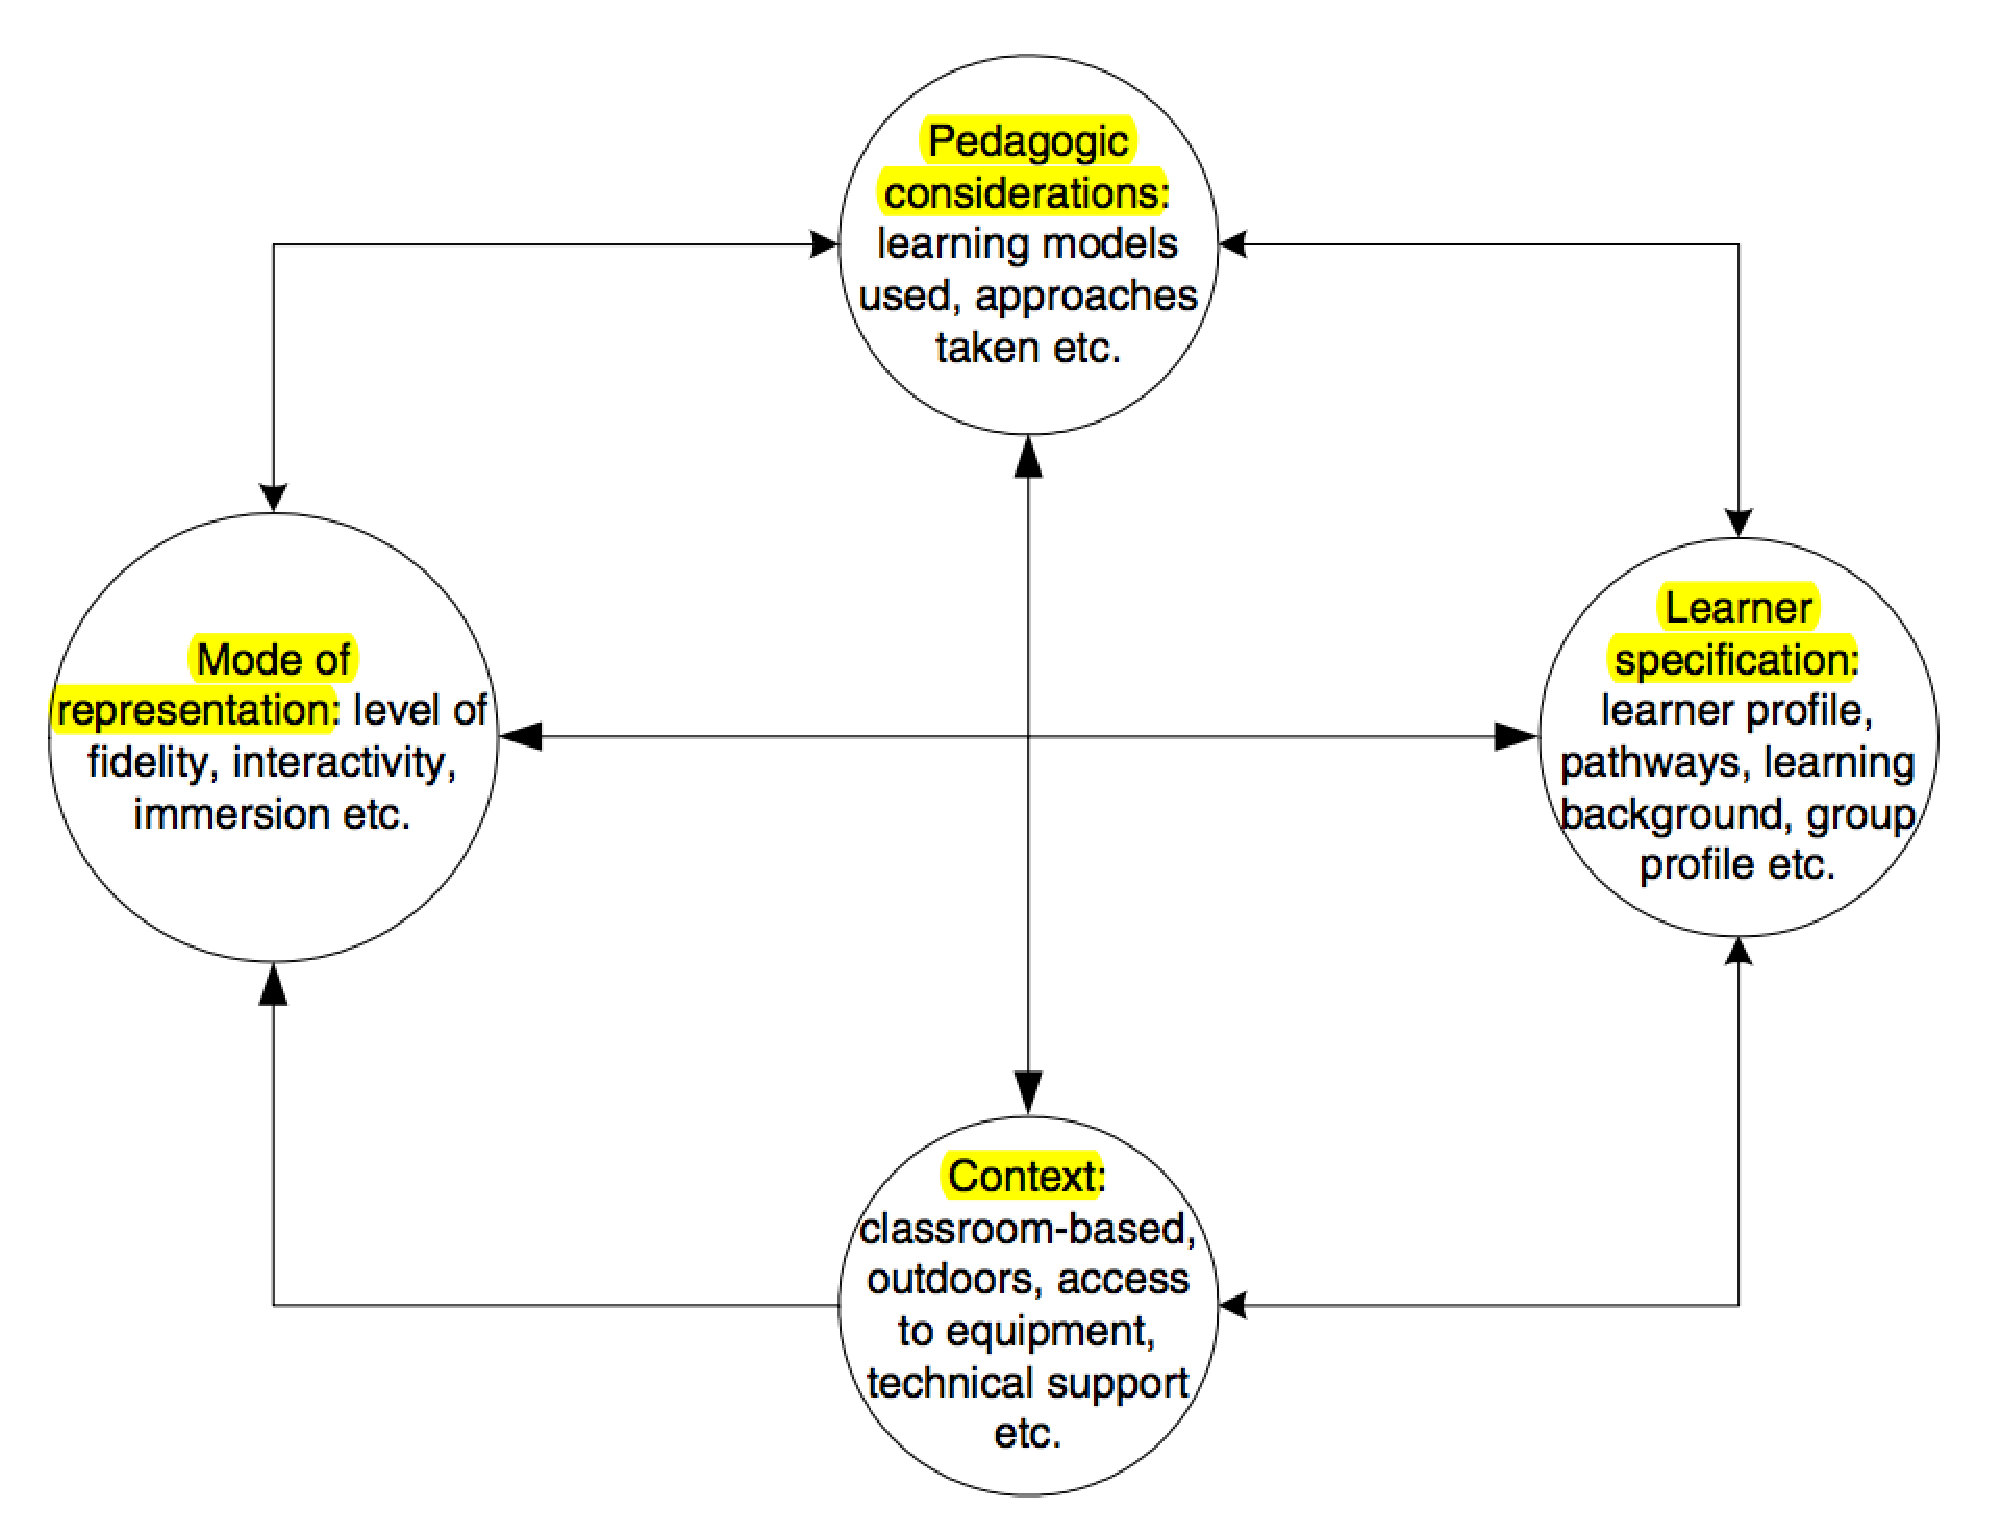
\includegraphics[width=0.7\columnwidth]{game-eval.eps}
		\caption{Four Dimensional Framework for Evaluating Educational Games \cite{de2006can}}
		\label{fig:four-dimensional-framework}
\end{figure}

Harteveld \cite{harteveld2010triadic} also agrees that ``Evaluatory research for games with a serious purpose is still at its infancy''. He proposes an evaluation framework called ``Triadic Game Evaluation (TGE)'' for assessing serious games. It consisting of three perspectives: Reality,
Meaning, and Play, as illustrated in the Figure \ref{fig:triadic-game-eval}.

\begin{figure}[htbp]
	\centering
		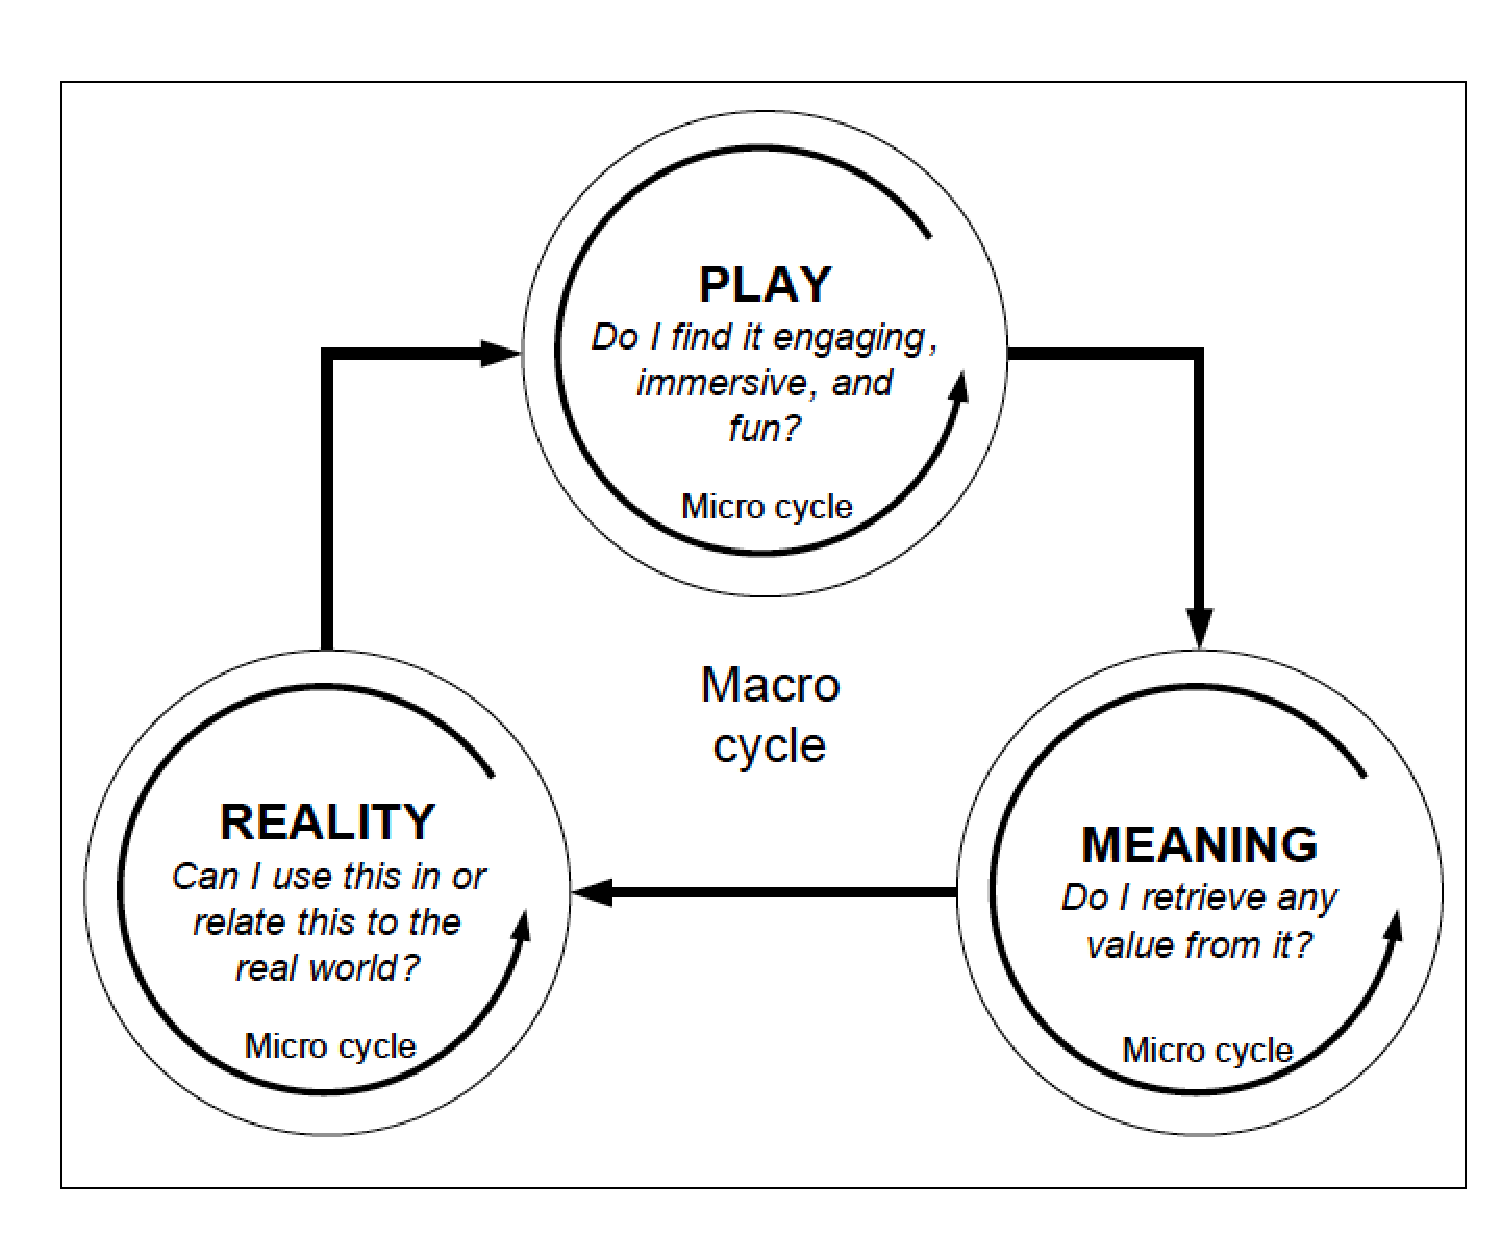
\includegraphics[width=0.7\columnwidth]{triadic-eval.eps}
		\caption{Triadic Game Evaluation (TGE) \cite{harteveld2010triadic}}
		\label{fig:triadic-game-eval}
\end{figure}

The above approaches focus on evaluation of a single game, as opposed to a game {\em
  framework}. One of the benefits of using a game framework is that, if correctly designed, it will provide useful and reusable ``building blocks'' with which to develop a variety of games. Yet how are we to know if a game framework has been ``correctly designed''?

Berger and Muller \cite {fabulaengine} describe their approach of using the Technology Acceptance Model (TAM) to evaluate the custom game engine Fabula \cite{fabula}. Technology Acceptance Model \cite {davis1986technology} is a well received theoretical model on assessing user acceptance of computer-based information systems, introduced by Fred Davis in his doctoral thesis in 1985. TAM considers that system use is a response that can be predicted by user motivation, which is influenced by an external stimulus of the system's features and capabilities. Figure \ref{fig:tam} illustrates the original Davis model. X1, X2 and X3 in the figure represent the system features.

\begin{figure}[htbp]
	\centering
		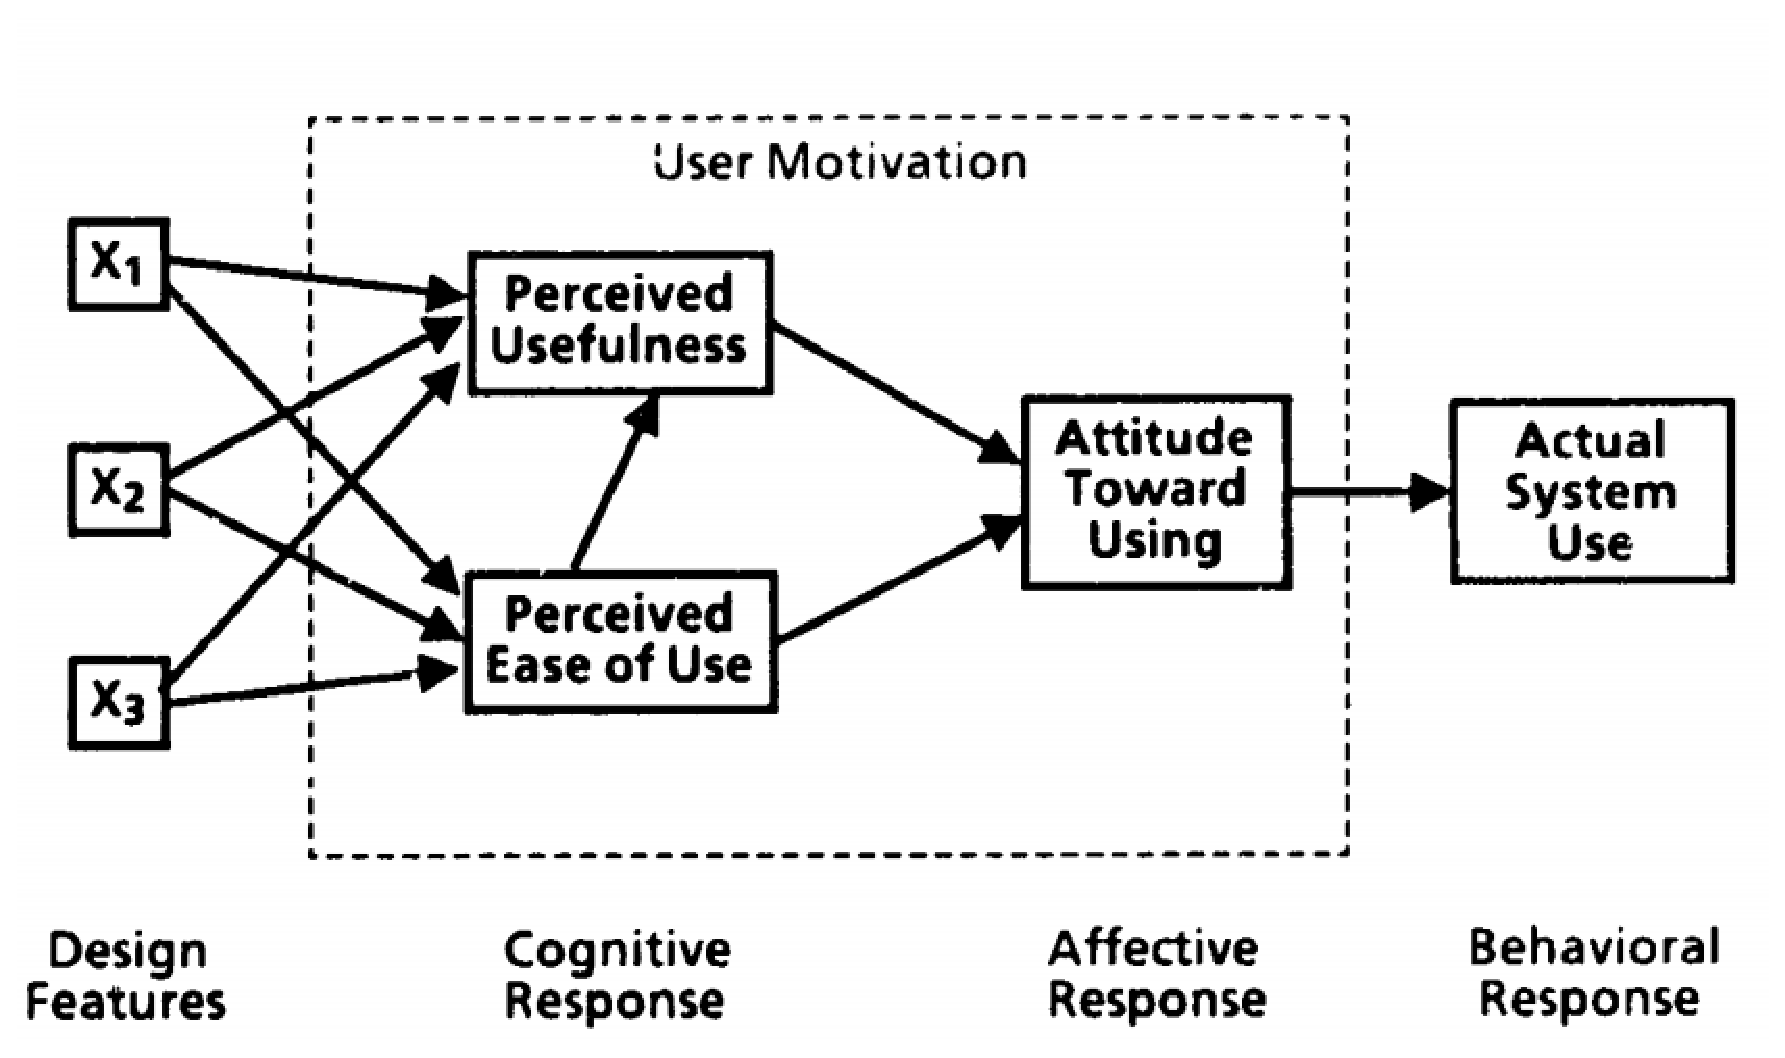
\includegraphics[width=0.7\columnwidth]{tam.eps}
		\caption{Technology Acceptance Model (TAM) \cite{davis1986technology}}
		\label{fig:tam}
\end{figure}

As Chuttur \cite{chuttur2009overview} points out in his review of TAM, there is  skepticism among some researchers regarding the rigor of the model. There exists  other assessment tools such as Game Engagement Questionnaire (GEQ) and Questionnaire for User Interaction Satisfaction (QUIS).  

Questionnaire for User Interaction Satisfaction (QUIS) \cite{harper1993improving} is a usability assessment tool developed in the HCI lab at the University Of Maryland, College Park. It is designed to assess user's subjective satisfaction regarding the human/computer interface of software systems. Currently licensing is required to access the QUIS questionnaires. 

Another usability assessment tool is the usability metrics described in Tullis and Albert 's book ``Measuring the User Experience'' \cite{tullis2010measuring}. For a usability procedure about completing transactions, Tullis and Albert suggest measuring task success, user efficiency, issues-based metrics, self-reported metrics, and live website metrics. Task success is a simple metric for a given task, does the user complete it or not? User efficiency is a measurement
of the effort required for the user to complete the task. For example, we can measure this by the amount of time spent to complete the task. Issues-based metrics involve measuring the number of times usability issues are encountered. Self-reported metrics are based on user responses to survey questions. Finally, live website metrics can be derived from analyzing the logs created by the website to understand the user experience.

Game Engagement Questionnaire (GEQ) \cite{brockmyer2009development} was developed by Brockmyer et al. and published in the Journal of Experimental Social Psychology. The questionnaire provides a ``psychometrically'' strong measure of levels of engagement specifically while playing video games. While the GEQ could measure the engagement level of positive game experience, the original intent of the research is to ``examine risk and protective factors for negative game impact''. Figure \ref{fig:geq} shows the questionnaire items.

\begin{figure}[htbp]
	\centering
		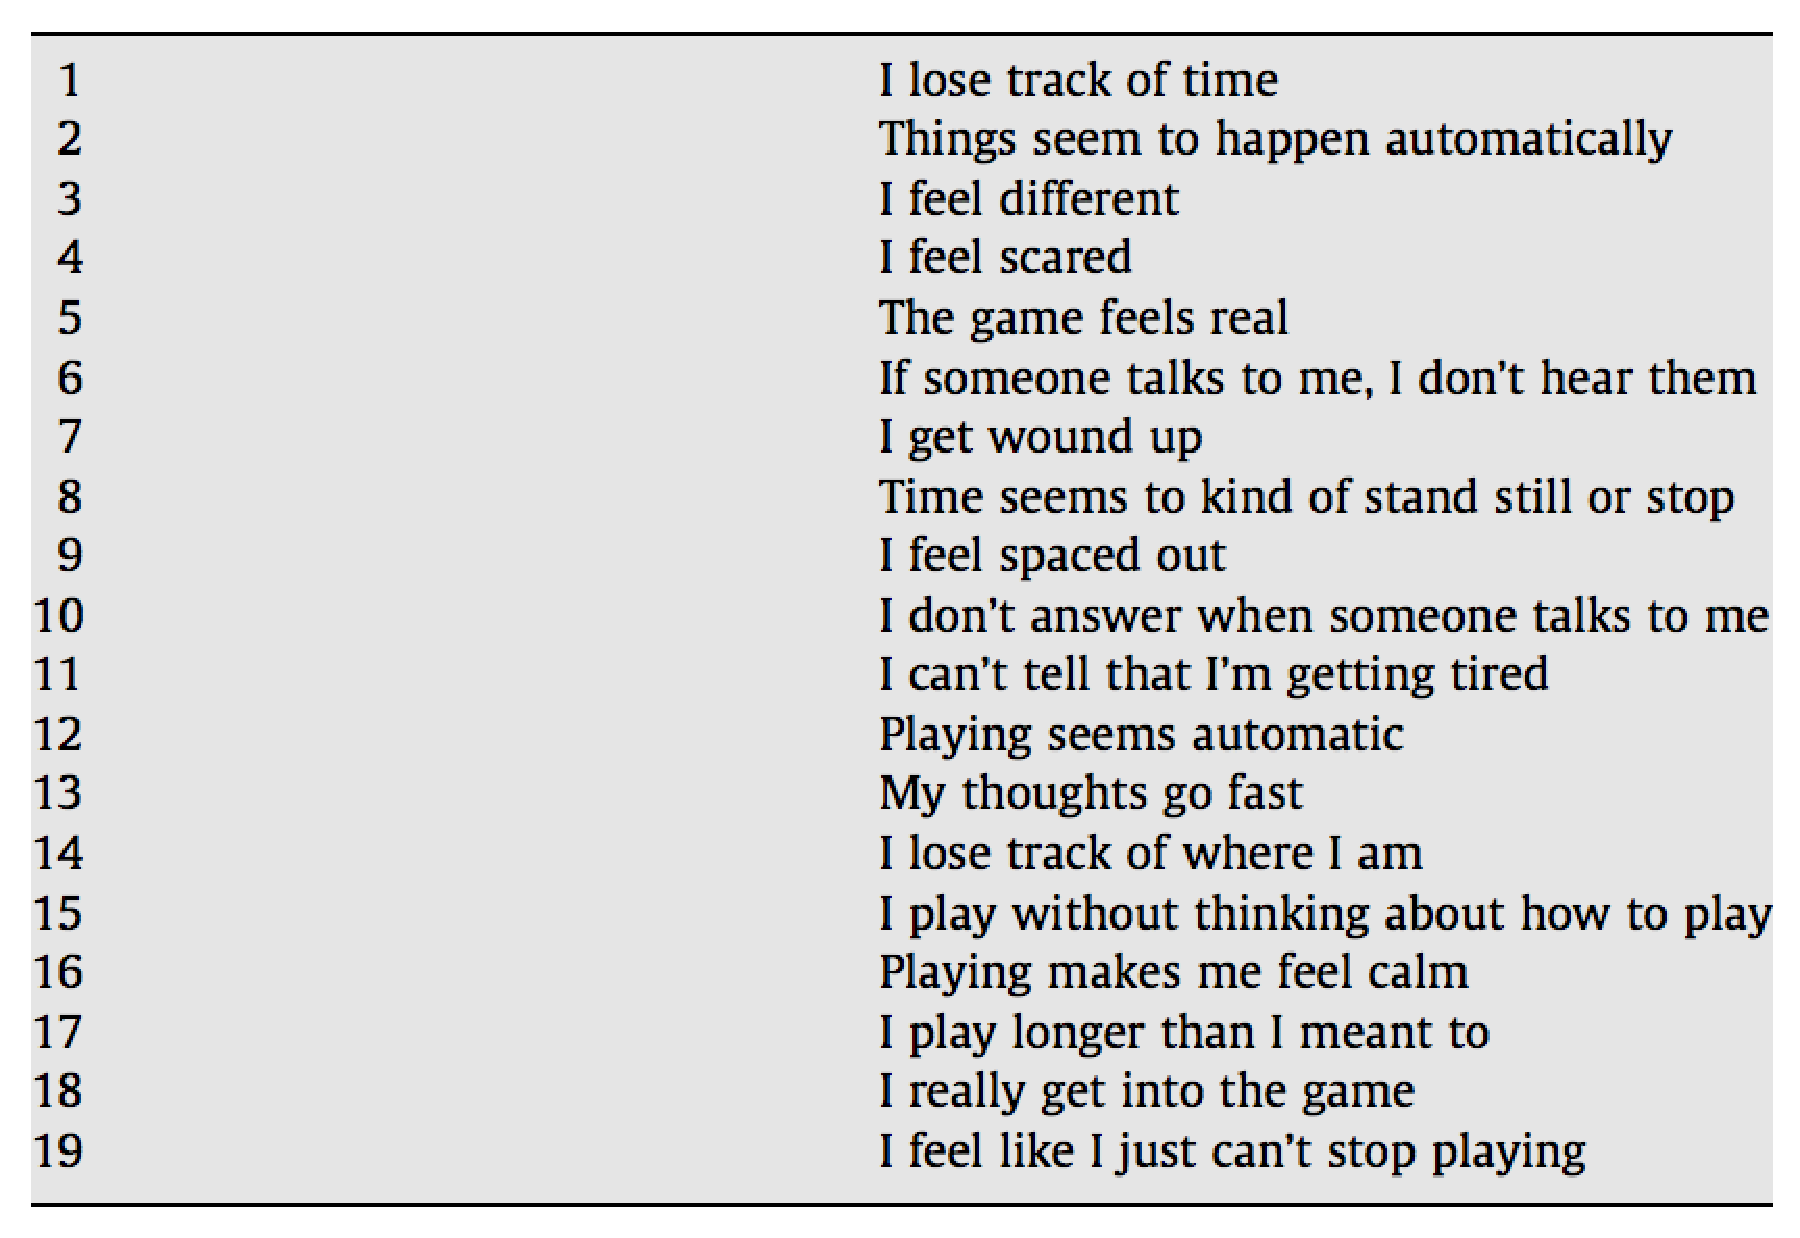
\includegraphics[width=0.7\columnwidth]{geq.eps}
		\caption{Game Engagement Questionnaire (GEQ) items \cite{brockmyer2009development}}
		\label{fig:geq}
\end{figure}

Ducheneaut et al. provides a good example of 
using game metrics for analysis of player's experience in a quantitative approach \cite {ducheneaut2006alone}. They reported the relationship of playing time and leveling in the MMORGs, as shown in \autoref{fig:player-metrics}:

\begin{figure}[htbp]
	\centering
		\subfigure[Average time required to reach a level]{\label{fig:metrics1}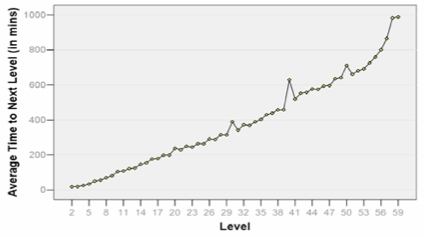
\includegraphics[height=1.7in]{metrics1.png}}
		\subfigure[Average accumulated play time by level]{\label{fig:metrics2}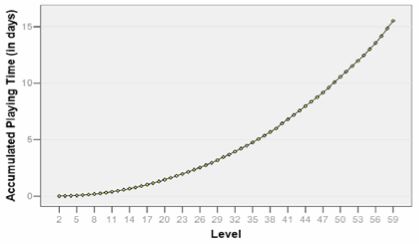
\includegraphics[height=1.7in]{metrics2.png}}
		\caption{Player Metrics (source: Ducheneaut \cite{ducheneaut2006alone})}
		\label{fig:player-metrics}
\end{figure}

Game metrics could be as important as creativity in game design. As Nadia Oxford points out, in the social game industry, player metrics collection and analysis are widely practiced to provide game designers to determine what the player audience likes and dislikes about a certain game experience \cite {Oxford2010}. 

E-Score is introduced by Gabe Zichermann, mainly applies in marketing gamification \cite {Petersen2011}. 
These are the metrics that go into the score:  
\begin{itemize}
  \item Recency : How long ago did they visit?  
  \item Frequency : How often did they come back? 
  \item Duration : How long did they stay? 
  \item Virality : How many people have they told about you? 
  \item Rating : What did they explicitly say when asked about you? 
\end{itemize}

Matt Fairchild lists and explains the basic terminology for social games metrics \cite {Fairchild2010}:

\textbf{ARPU}: Average Revenue Per User (ARPU) is measured as total revenue divided by the number of subscribers. This includes revenue from subscriber fees, virtual goods, affiliate marketing and ad impressions. Because social games are so metrics-heavy, ARPU can be broken down by day, by country, by demographic, or by pretty much any other metric.

\textbf{Churn}: The turnover rate (or �attrition rate�) of a social game�s active players. Churn refers to the constant loss and gain of members, especially high in casual gaming.

\textbf{Cohort}: Cohorts are used for analyzing retention. By organizing users in groups such as ``everyone that visited on June 10th'' and analyzing the percentage that revisit, you can pinpoint what promotions are having the greatest effect.

\textbf{DAU}: Daily Active Users (DAU) is the number of active users over the course of a single day.

\textbf{DAU/MAU}: Comparing Daily Active Users to Monthly Active Users shows roughly how many days per month the average user engages with a game. The DAU/MAU ratio is strongly correlated with social gaming success.

\textbf{Engagement}: Engagement measures how long users spend playing a game. How many features do they access? Are they spending hours or seconds? How many pages does the average user view? What percentage are returning visitors?

\textbf{Entry Event}: An entry event is the first action a user performs when he  enters the game. What do users do first? Which entry events are the most effective at bringing people back? By determining the more popular entry events, you can push more resources towards them, thus increasing retention, engagement and re-engagement.

\textbf{Exit Event}: Exit events are the last actions a user performs before exiting the game. Tracking the Exit Event Distribution helps show why users are disengaging with the game.

\textbf{K Factor}: K Factor measures the virality of a game. K Factor = (Infection Rate) * (Conversion Rate). An Infection Rate is how much a given user exposes the game to other players, such as through status updates or email invites. A conversion rate is when that ``infection'' results in a new sign up. A high K Factor indicates effectiveness of bringing in new players.

\textbf{Lifetime Network Value}: The value a user provides to your network over the course of his entire ``lifetime'' on the network. For instance, is the user contributing to viral effects, evangelizing the game or contributing positively to ARPU? This is compared to the User Acquisition Cost, or how much it costs (via marketing and viral efforts) to bring in new members.

\textbf{MAU}: Like DAU, Monthly Active Users (MAU) tracks the total number of users in a given month.

\textbf{Re-Engagement}: Re-engagement is about how to get users back. It includes re-engaging gamers who have been signed off for an hour, a day, a month, or more. 

\textbf{Retention}: Retention is how well you maintain user base, as the opposite of churn. 
\\\\
Appdata.com gathers independent application metrics from most of the social game application. For example, the graphs in \autoref{fig:social-game-metrics} shows the DAU (Daily Active User) and MAU (Monthly Active User) metrics for the popular Farmville social game \cite {appdata2011}:

\begin{figure}[htbp]
	\centering
		\subfigure[FarmVille DAU]{\label{fig:farmville1}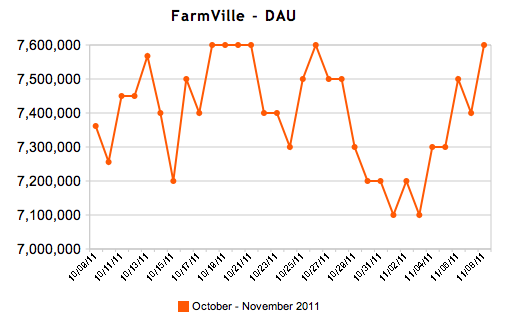
\includegraphics[height=1.85in]{FarmVille2.png}}
		\subfigure[FarmVille MAU]{\label{fig:farmville2}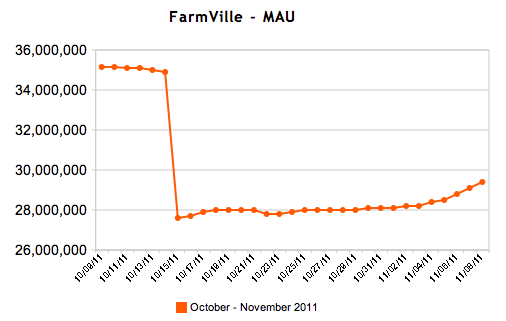
\includegraphics[height=1.85in]{FarmVille1.png}}
		\subfigure[FarmVille DAU/MAU]{\label{fig:farmville3}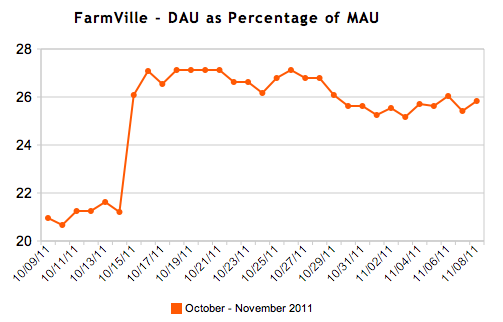
\includegraphics[height=1.85in]{FarmVille3.png}}
		\caption{Social Game Metrics (source: Appdata.com \cite {appdata2011})}
		\label{fig:social-game-metrics}
\end{figure}

Kontagent, a user analytics service company, introduces the top 10 social game metrics \cite {Kontagent2010}: (1) Entry Event Distribution. (2) Outbound Messages/User. (3) Viral Message CTR/Conversion. (4) Virality (K-factor). (5) Engagement. (6) Exit Event Distribution. (7) Retention - Revisit Rate. (8) Lifetime Network Value. (9) Conversion to paying users. (10) Average Revenue Per Paying User.

\section{Summary}
\label{sec:rel-summary}

In summary, this chapter discusses related work on serious games and gamification, game design thinking, serious games for sustainability, serious game framework and its assessment.

The above assessment framework or tools are for general purpose. From my literature search, I have not yet found any prior work concerning the comprehensive approach for the particular needs of a serious game framework assessment. 